%! Author = PERSON
%! Date = DATE


\documentclass[11pt, a4paper]{report}

% Listings
\usepackage{listings}

\lstset{
    literate={ö}{{\"o}}1
        {ä}{{\"a}}1
        {ü}{{\"u}}1
}

\lstset{language=Java,
    basicstyle=\ttfamily,
    keywordstyle=\color{javapurple}\bfseries,
    stringstyle=\color{javared},
    commentstyle=\color{javagreen},
    morecomment=[s][\color{javadocblue}]{/**}{*/},
    numbers=left,
    numberstyle=\tiny\color{black},
    stepnumber=2,
    numbersep=10pt,
    tabsize=4,
    showspaces=false,
    showstringspaces=false}

% Packages
\usepackage[margin=1.4in]{geometry}
\usepackage[T1]{fontenc}
\usepackage[utf8]{inputenc}
\usepackage[ngerman]{babel}
\usepackage{hyperref}
\usepackage{verbatim}
\usepackage{graphicx}
\usepackage{float}
\usepackage{pdfpages}
\usepackage[
    singlelinecheck=false
]{caption}
\usepackage[raggedright]{titlesec}
\usepackage[nottoc]{tocbibind}
\usepackage{longtable}
\usepackage{tocloft}
\usepackage{fancyhdr}
\usepackage{lastpage}
\usepackage{pifont}
\usepackage{amsmath}

\usepackage[automake]{glossaries-extra}
\usepackage{wasysym}
\usepackage{textcomp}
\usepackage{color}
\usepackage{graphicx}
\usepackage[paper=portrait,pagesize]{typearea}
\usepackage{pdfpages}
\usepackage{pdflscape}



\titleformat{\chapter}{\normalfont\bfseries\LARGE\raggedright}{\thechapter}{1ex}{}
\titlespacing*{\chapter}{0pt}{30pt}{30pt}
\setcounter{secnumdepth}{3}
\setcounter{tocdepth}{3}
\setlength{\cftsecnumwidth}{2.8em}
\renewcommand\labelitemi{$-$}
\renewcommand\labelitemii{$-$}
\renewcommand\labelitemiii{$-$}
\renewcommand{\headrulewidth}{0pt}

\usepackage[
    backend=biber,
]{biblatex}
\addbibresource{global/quellens.bib}

\usepackage[toc]{glossaries}
\makeglossaries
\loadglsentries{global/glossar_eintraege}

\pagestyle{fancy}
\fancyhf{}
\renewcommand{\headrulewidth}{0pt}
%TODO Platzhalter ersetzen
\lfoot{\fontsize{10}{15} \selectfont Niculin Steiner}
\cfoot{\fontsize{10}{15} \selectfont \today}
\rfoot{\fontsize{10}{15} \selectfont \thepage~von~\pageref*{LastPage}}
\fancypagestyle{plain}{}

\newcommand{\oksymbol}{{\color{green}\ding{51}}}
\newcommand{\errorsymbol}{{\color{red}\ding{55}}}

\makeatletter
\def\blx@citation#1#2{\blx@citation@entry{#1}{#2}}
\makeatother
\renewcommand{\arraystretch}{1.5}
% Document
\begin{document}

    \begin{titlepage}

    \begin{figure}
        \begin{center}
            
\includegraphics[width=0.6\textwidth]{ressourcen/ergon_logo_gross}
            \captionsetup{textformat=empty, labelformat=empty}
            \caption[Logo der Ergon Informatik AG]{Logo der Ergon Informatik AG}\label{fig:ergon-logo-gross}
        \end{center}\nocite{ergonlogo}
    \end{figure}
    \begin{center}
        \vspace*{2cm}
        \Huge
        \textbf{Probe-IPA}

        \vspace{0.5cm}
        \Large

Erweiterung in der Airlock IAM Adminapp im Bereich 2FA um Aktivierungscode anzuzeigen

        \vfill

        \Large
        Probe-IPA von Niculin Steiner

        \vspace*{3cm}

        \large
        Ergon Informatik AG\\
        \today\\

    \end{center}
\end{titlepage}

    \renewcommand*\contentsname{Inhalt}
\tableofcontents

    \part{Umfeld und Ablauf}\label{part:1}
    \chapter{Aufgabenstellung}\label{ch:aufgabenstellung}
In diesem Kapitel sind die Aufgabenstellung und die Rahmenbedingungen aufgeführt. Der grösste Teil des Inhalts stammt aus der originalen Aufgabenstellung.


\section{Ausgangslage}\label{sec:ausgangslage}
Airlock Identity and Access Management (IAM) ist ein bestehendes, in unserer Abteilung entwickeltes Produkt, das unter anderem Logins (Authentisierungen) ermöglicht. Eine weitere Funktionalität eines IAMs ist der Admin-Bereich (adminapp). Airlock IAM unterstützt unterschiedliche Stufen von Administratoren, um beispielsweise Mitarbeitenden im Support oder an einem Kundenschalter spezifisch eingeschränkten Zugriff für die Verwaltung von Usern zu erlauben.\newline\newline
Airlock 2FA erlaubt es, nebst beispielsweise Usernamen und Passwort, einen weiteren Authentisierungsfaktor zu verwenden. Üblicherweise wird dazu die Airlock 2FA App auf dem Smartphone installiert und aktiviert.\newline
Es gibt mehrere Möglichkeiten, wie Kund:innen für den eigenen Login die Airlock 2FA aktivieren können. Ein Weg ist beispielsweise über einen Brief mit einem QR Code, welchen Kund:innen dann mit der Airlock 2FA App scannen können. Die Aktivierung ist auch über einen 16-stelligen Aktivierungscode möglich.\newline\newline
Immer wieder kommt es vor, dass Kund:innen Unterstützung bei der Aktivierung von Airlock 2FA benötigen und sich telefonisch beim Firmen-Helpdesk oder am physischen Schalter melden. Damit das Support- oder Schalterpersonal der Kundschaft helfen kann, die Airlock 2FA zu aktivieren, braucht es eine Möglichkeit, den 16-stelligen Aktivierungscode für den spezifischen User anzuzeigen.\newline
Bisher gibt es in Airlock IAM noch kein Feature, damit der Administrator-Bereich solche 16-stelligen Aktivierungscodes pro User anzeigen kann. \pagebreak

\section{Detaillierte Aufgabenstellung}\label{sec:detaillierte-aufgabenstellung}
\subsection*{Ziele}
\begin{itemize}
	\item UC1: Helpdesk kann Kunden am Telefon helfen, ein Gerät zu aktivieren.
	\item UC2: Schaltermitarbeiter kann Kunde am Schalter helfen, ein Gerät zu aktivieren
	\item UC3: Es soll möglich sein, den Zugriff auf die userspezifischen 16-stelligen Aktivierungscodes nur für bestimmte Administratoren-Rollen (bspw. Rolle Helpdesk) freizugeben, damit nicht alle Administratoren sich den 16-stelligen Aktivierungscode anzeigen lassen können.
	\item UC4: Im User Activities Logfile des spezifischen Users soll geloggt werden, welcher Administrator-Account zu welchem Zeitpunkt den 16-stelligen Aktivierungscode angezeigt hat, damit im Nachhinein nachvollziehbar ist, welche Administratoren je Zugriff auf den Aktivierungscode hatten.
\end{itemize}

\subsection*{Weitere Anforderungen}
\begin{itemize}
	\item Der Code soll auf Knopfdruck in der Adminapp angezeigt werden. Dabei sind UI-Komponenten zu verwenden, die an anderen Stellen in der Adminapp auch schon verwendet werden. Eine mögliche Lösung ist ein SPA Popup (kein Browser Popup) mit einem 'Schliessen' Knopf.
	\item Neue Plugins oder Plugin Properties sollen einen klaren und vollständigen Hilfetext haben.
\end{itemize}

\subsection*{Erwartete Artefakte}
Nebst der IPA Dokumentation werden diese technischen Artefakte erwartet:
\begin{itemize}
	\item Sinnvolles Slicing und Anzahl von Gerrit Changes mit der implementierten Lösung und Git Kommentaren, die unseren internen Konventionen entsprechen. Der Kandidat entscheidet selbst, wie viele Gerrit Changes sinnvoll sind. Er hat dabei zu beachten, dass die Changes aufeinander aufbauen sollten und \flqq verdaubare\frqq{} Review-Grössen haben.
	\item Beschreibung wie das neue Feature konfiguriert werden kann in der Airlock IAM Kundendokumentation. Dazu soll das Kapitel 18.5 Airlock 2FA configuration sinnvoll erweitert werden. Die angepasste Kundendokumentation soll auf Englisch und in den restlichen PDF-Unterlagen enthalten sein (es ist nicht nötig, mit unserem Kundendokumentation-Tool SMC zu arbeiten).
\end{itemize}

\subsection*{Abgrenzung}
\begin{itemize}
	\item Administratoren können pro User bereits Aktivierungsbriefe erstellen oder anfordern. An dieser Logik soll im Rahmen dieses Issues nichts verändert oder erweitert werden.
\end{itemize}




\section{Mittel und Methoden}\label{sec:mittel-und-methoden}

Es wird auf dem aktuellen Stand der Entwicklung von Airlock IAM 8.4 aufgebaut.

\subsection*{REST Technologien}
\begin{itemize}
	\item Java(Guice als Dependency Injection Framework), JSON, JUnit
	\item Jackson, Jersey, Guice
	\item REST Integration Tests
\end{itemize}

\subsection*{SPA Technologien}
\begin{itemize}
	\item Angular (Typescript/RXJS)
	\item Bootstrap (HTML/CSS/SASS)
	\item Selenium UI Testing
\end{itemize}

\subsection*{Wichtigste Tools}
\begin{itemize}
	\item Intellij(IDE)
	\item Gerrit + Git (SCM)
\end{itemize}



\section{Vorkenntnisse}\label{sec:vorkenntnisse}
Der Kandidat war involviert in die Implementation von SPA und REST Features im Bereich IAM Protected Self-Service. \newline
Das Grundgerüst der SPA und REST Endpunkte ist bekannt.


\section{Vorarbeiten}\label{sec:vorarbeiten}
    Der Kandidat hat für die Probe-IPA keine vorbereiteten Tätigkeiten erarbeitet, hat sich aber in das Thema Airlock 2FA eingelesen.
\section{Neue Lerninhalte}\label{sec:neue-lerninhalte}
Erfahrung bei der selbständigen Entwicklung einer produktrelevanten Erweiterung unter realistischen Bedingungen.
\begin{itemize}
\item Futurae API: \url{https://www.futurae.com/docs/api/auth/} 
\item IAM Kunden Dokumentation: \url{https://docs.airlock.com/iam/8.3/}´
\end{itemize}

\section{Arbeiten in den letzten 6 Monaten}\label{sec:arbeiten-in-den-letzten-6-monaten}
In den letzten sechs Monaten hat der Kandidat Erfahrungen in folgenden Bereichen gesammelt:
\begin{itemize}
    \item OAuth 2.0 / OpenID Connect Consent Management Self-Service, SPA und REST
    \item Have I Been Pwnd Scriptable Step, 3rd Party REST API, Lua
    \item HTTP Cache Control Konfiguration im Zusammenhang mit JWKS REST Endpoint
\end{itemize}

    \chapter{Projektaufbauorganisation}\label{ch:projektaufbauorganisation}

Die folgenden Personen sind in dieses Projekt involviert:
\renewcommand{\arraystretch}{1.5}
\begin{longtable}{|p{.30\textwidth}|p{.30\textwidth}|p{.40\textwidth}|}
    \hline
    \textbf{Person}                 & \textbf{Rolle}                 & \textbf{Aufgabe/Verantwortung}                                                                                                                   \\
    \hline
    \hypertarget{k}{Niculin Steiner}         & Kandidat (K)                   & Umsetzen der Facharbeit                                                                                                                          \\
    \hline

    \hypertarget{vf}{Pascal Knecht}     & Verantwortliche Fachkraft (VF) & Facharbeit begleiten, technische Fragen beantworten, Bewertung der Facharbeit                                                                    \\
    \hline

    \hypertarget{hex}{Bernd Lienberger}      & Hauptexperte (HEX)             & IPA bezogene Fragen beantworten, Entscheiden bei auftretenden Problemen, Besuchstermine festlegen, Fachgespräch leiten, Bewertung der Facharbeit \\
    \hline
\end{longtable}
\renewcommand{\arraystretch}{1}

    \chapter{Benützte Firmenstandards}\label{ch:benuetzte-firmenstandards}

Für die Umsetzung diser Probe-IPA wurde für den Bericht und den Zeitplan eine Vorlage verwendet.

    \chapter{Arbeitsumgebung}\label{ch:arbeitsumgebung}
In diesem Abschnitt wird der Arbeitsplatz und die Umgebung, während der Probe-IPA, des Kandidaten beschrieben.
\section{Arbeitsplatz}\label{sec:arbeitsplatz}

\begin{figure}[H]
    \begin{center}
        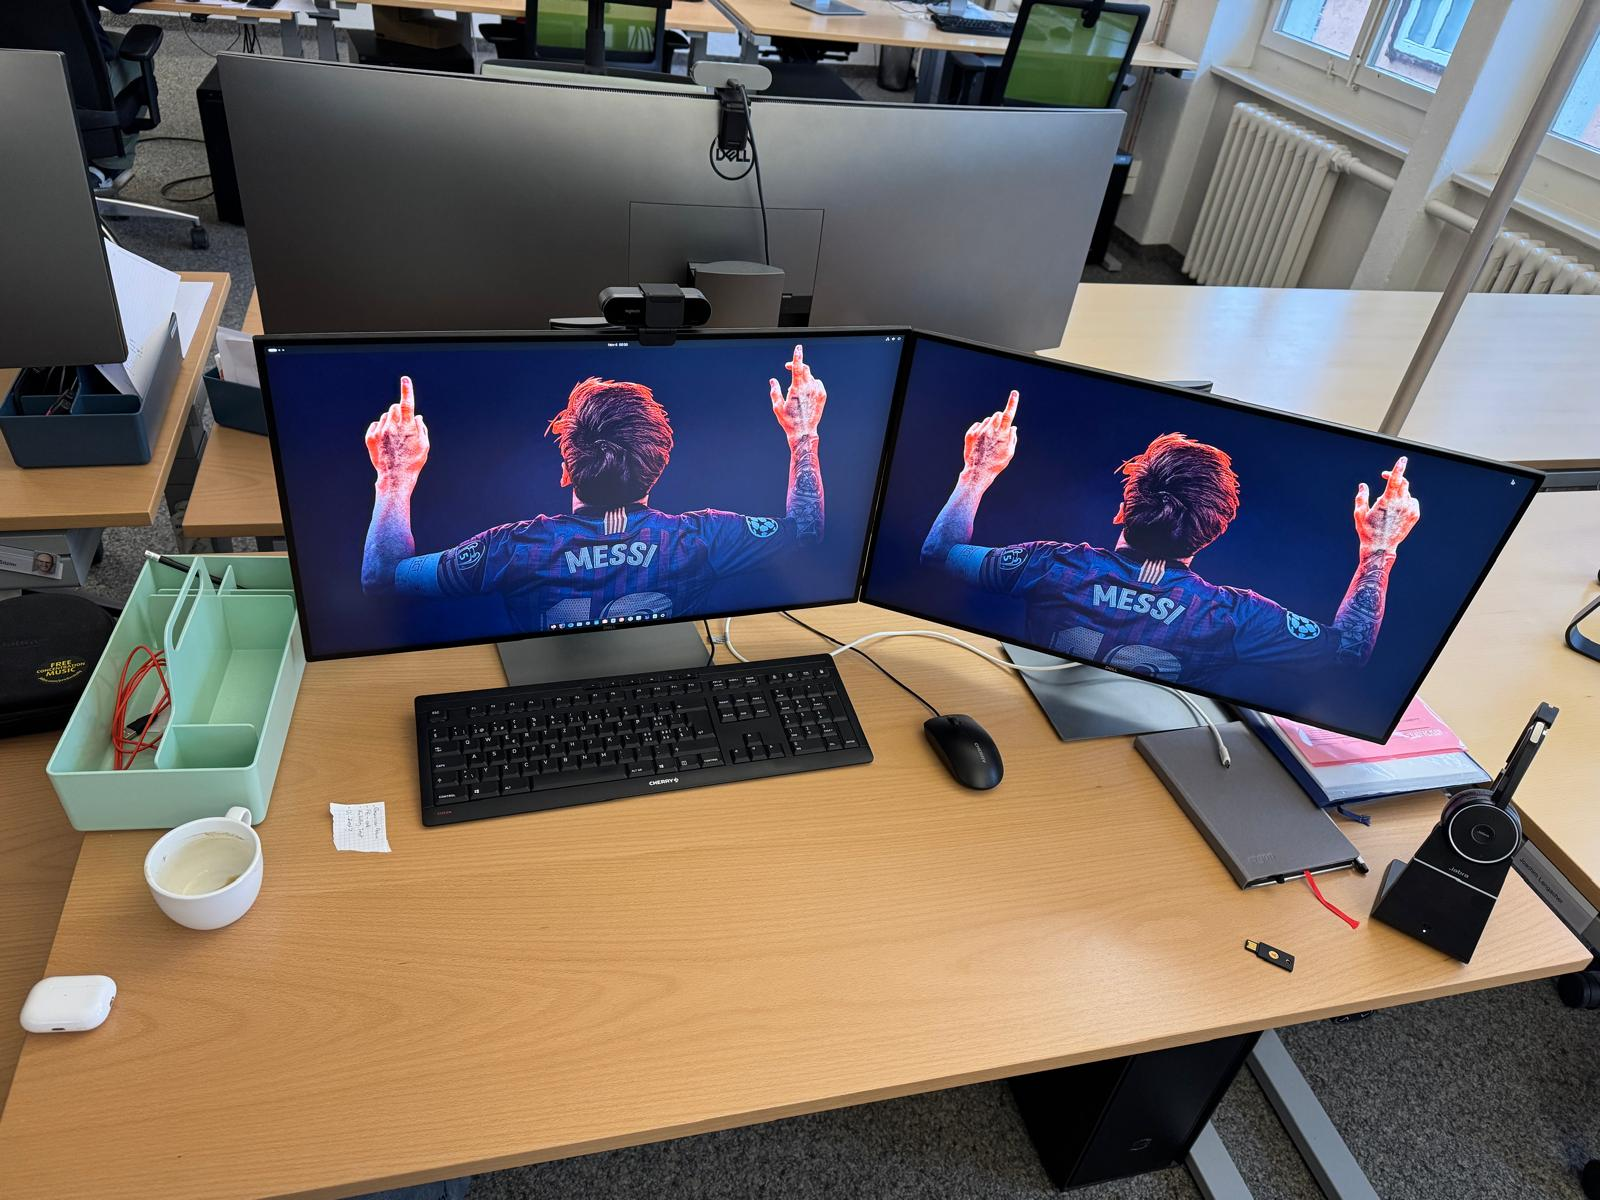
\includegraphics[width=0.8\textwidth]{ressourcen/arbeitsplatz}
        \caption[Arbeitsplatz]{Arbeitsplatz während der Probe-IPA}\label{fig:arbeitsplatz}
    \end{center}
\end{figure}

Da seit der Mitarbeit im IAM nie im Homeoffice gearbeitet wurde, findet auch die Probe-IPA wie gewohnt vor Ort statt. Der Desktop PC mit dem Betriebssystem Linux (Distribution Ubuntu) ist für die maximale Effizienz mit 2 Bildschirmen verbunden. Um im Grossraumbüro möglichst ungestört zu arbeiten, liegen dem Kandidaten ein Paar Airpods Pro mit Noise Cancelling vor.

\newpage \section{Verwendete Tools}\label{sec:verwendete-tools}
Die folgende Tabelle zeigt einen Überblick der wichtigsten Tools, welche für die Umsetzung der Probe-IPA verwendet wurden:

\renewcommand{\arraystretch}{1.5}
\begin{longtable}{|p{.22\textwidth}|p{.40\textwidth}|p{.38\textwidth}|}
    \hline
    \textbf{Tool} & \textbf{Einsatzzweck} & \textbf{Link} \\ \hline
    Intellij Ultimate           & Entwicklungsumgebung, zur Entwicklung des Features                   & \url{https://www.jetbrains.com/de-de/idea/}     \\ \hline
    TeXstudio           & Enticklungsumgebung für Latex, mit welchem die Dokumentation geschrieben wurde & \url{https://www.texstudio.org/}     \\ \hline
    Gerrit           & Quellcode Verwaltung & \url{https://www.gerritcodereview.com/}     \\ \hline
    Git          & Versionskontrollsystem & \url{https://git-scm.com/}     \\ \hline
    Jenkins & Automatisierte Testruns  & \url{https://www.jenkins.io/}     \\ \hline
    Outlook & Termin für den Expertenbesuch im Blick behalten& \url{https://www.microsoft.com/de-ch/microsoft-365/outlook} \\ \hline
    Postman & Testen der eigenen API und der API von Futurae & \url{https://www.postman.com/} \\ \hline
    LibreOffice & Erstellen und warten des Zeitplans & \url{https://de.libreoffice.org/} \\ \hline
    Github & Backup und Versionierung des Berichts und des Zeitplans & \url{https://github.com/} \\ \hline
    Gliffy & Diagramme \& Mockups erstellen & \url{https://www.gliffy.com/} \\ \hline
    Mockito & Mocking für Unit-Tests& \url{https://site.mockito.org/} \\ \hline
    JUnit5 & Testframework für Java & \url{https://junit.org/junit5/} \\ \hline
    Selenium & Framework für automatisierte Softwaretests von Webanwendungen  & \url{https://www.selenium.dev/} \\ \hline
    Wiremock & Simulieren des Futurae Server für Unittests & \url{https://www.wiremock.io/} \\ \hline    
\end{longtable}
\renewcommand{\arraystretch}{1}
\newpage
    \chapter{Versionierung und Sicherung der Arbeitsergebnisse}\label{ch:versionierung-und-sicherung-der-arbeitsergebnisse}

Die Arbeitsergebnisse sollten gesichert werden. Damit, im Falle eines unerwarteten Ausfalls während der Probe-IPA, z.B des Rechners, von einem anderen Gerät wieder auf den Stand zugegriffen werden kann. Zu dem sollte es generell möglich sein jeder Zeit auf einen älteren Stand zurück zukommen.

\section{Git als Versionierungstool}
Für die Versionierung der Arbeitsergebnisse wurde Git verwendet. 
Git ist weit verbreitet und ist auch aus der Schule und diversen anderen Projekten bekannt. Es wird verwendet um Änderungen am Code zu verfolgen und erstellt dabei eine Versionshistorie. 

\section{Git im Zusammenspiel mit Gerrit}
Der Quellcode liegt in einem Git-Repository auf Gerrit. Gerrit dient dazu als Review und Code Management Tool. 
Im Vergleich zur \flqq gewöhnlichen\frqq{}  Entwicklung mit Git, bei der man für neue Features Branches und Commits erstellt arbeitet man bei Gerrit sozusagen auf Commmitbasis. 
Pusht man einen neuen Commit auf Gerrit, erstellt dieser ein neues\flqq Changeset\frqq{}  mit einem Patchset. Gibt es nun weitere Änderungen werden diese einfach Amandet, dies erstellt dann ein weiters Patchset in diesem Changeset. Für grössere und komplexere Änderungen können auch aufeinander aufbauende Changesets erstellt werden. 

    
\chapter{Projektmanagementmethode}\label{ch:projektmanagementmethode}

In diesem Kapitel wird die Projektmanagementmethode IPERKA beschrieben. Es wird dargelegt wieso diese Methode gewählt wurde und was die Vor und/oder Nachteile daran sind.

\section{IPERKA}\label{sec:iperka}

Für die Probe-VA wurde IPERKA als Projektmanagementmethode gewählt. Sie eignet sich gut für kleine Projekte. Sie lassen sich damit einfach und strukturiert planen sowie umsetzen. 
Die IPERKA Methode setzt sich aus folgenden 6 Schritten zusammen:

\subsection{Informieren}
Der erste Punkt bei IPERKA ist das Informieren. Dabei wird sich ein Überblick über das Projekt / den Projektauftrag verschaffen. Es gilt zu klären was genau der Auftrag ist, und ob alle Informationen vorhanden sind.

\subsection{Planen}
Als zweiten Schritt kommt das Planen. Hier wird das Projekt konkreter und es wird ein Zeitplan erstellt. Und je nach Team grösse, werden bestimmte Aufgaben zugeteilt. Im Probe-IPA Fall fällt dies natürlich weg.

\subsection{Entscheiden}
Beim Entscheiden, wird entschieden welchen Lösungsweg gegangen werden soll. Es wird z.B definiert mit welchen Tools / Technologien gearbeitet wird. Wichtig ist auch, dass die Kriterien, welche zu dieser Entscheidung geführt haben, definiert werden.

\subsection{Realisieren}
In diesem Teil geht es an die Umsetzung. Das Projekt wird nach dem definierten Plan sowie Zeitplan versucht umzusetzen.

\subsection{Kontollieren}
Der fünfte Schritt erfolgt teilweise parallel zum Vierten. In diesem Schritt wird von oben auf das laufende Projekt geblickt und geschaut, ob alles nach Plan läuft. Gibt es Abweichungen und falls ja, können diese begründet werden?

\subsection{Auswerten}
Der letzte Schritt dient dazu, nochmals auf das Projekt zurückzublicken und es zu Reflektieren.

\section{Alternative Methode - Scrum}\label{sec:alternative-methode}
Nebst IPERKA gibt es auch noch andere Alternativen. Eine davon ist Scrum. 
Scrum eignet sich allerdings nicht besonders für die Umsetzung eines Projekts wie die Probe-IPA.  Sie ist eine Agile Projektmanagementmethode, welche sich für Projekte eignet, die sehr dynamisch und doch komplex sind. Meistens sind die konkreten Anforderungen zu Beginn sogar noch unklar. Zudem kann Scrum nur teilweise alleine durchgeführt werden.
Dies ist bei der Probe-IPA nicht der Fall. Deshalb wurde sich für IPERKA entschieden.
    \chapter{Arbeitsprotokoll}\label{ch:arbeitsprotokoll}
\renewcommand{\arraystretch}{1.5}
\begin{longtable}{p{.22\textwidth}|p{.78\textwidth}}
    \hline
    \textbf{Datum}                       & 06.11.2024\\
    \hline
    \textbf{Bearbeitete Arbeitspakete}   & 1.1, 1.2, 2.1, 2.2, 7.1, 7.2, 7.3\\
    \hline
    \textbf{Arbeitszeit}                 & 8h \\
    \hline
    \textbf{Überzeit}                    & 0 \\
    \hline
    \textbf{Vergleich mit dem Zeitplan}  & Da ich den Zeitplan noch nicht fertig erstellt habe, kann ich für heute keinen Vergleich ziehen. \\
    \hline
    \textbf{Erfolge und Probleme}        & Zu Beginn wusste ich nicht genau wie ich am besten vorgehe resp. was ich zuerst angehe, da hat mir das vorhandene Template einen sehr guten Leitfaden gegeben. Und so habe ich begonnen alles der Reihe nach auszufüllen/ zu dokumentieren. Und bin am Schluss weiter gekommen als gedacht.\\
    \hline
    \textbf{Tagesreflexion}              & Heute bin ich sehr gut voran gekommen. Ich konnte bereits den Teil 1 der Dokumentation abschliessen und mit den Arbeitspaketen beginnen.
    \\
    \hline
    \textbf{In Anspruch genommene Hilfe} & Fragen an Pascal bezüglich der Aufgabenstellung. War mir unsicher, wo genau die Kundendoku hin muss. Jetzt weiss ich, dass es reicht, wenn ich sie im Anhang anhänge.\\
    \hline
\end{longtable}\label{tab:arbeitsprotokoll-tag1} 

\newpage

\begin{longtable}{p{.22\textwidth}|p{.78\textwidth}}
	\hline
	\textbf{Datum}                       & 07.11.2024 \\
	\hline
	\textbf{Bearbeitete Arbeitspakete}   & 2.1, 2.2, 2.3, 2.4 \\
	\hline
	\textbf{Arbeitszeit}                 & 8h \\
	\hline
	\textbf{Überzeit}                    & 0 \\
	\hline
	\textbf{Vergleich mit dem Zeitplan}  & Eine Stunde voraus \\
	\hline
	\textbf{Erfolge und Probleme}        & Beim Zeitplan hatte das Template nicht richtig funktioniert. Da kam ein bisschen extra Aufwand dazu, da ich aber ansonsten etwas schenller war hat sich das wieder Kompensiert. Ich konnte bereits heute mit dem SPA Lösungskonzept beginnen. Da gestern der Zeitplan noch nicht stand, erwähne ich es heute: Ein weiterer Erfolg, ich konnte
Meilenstein A (Informieren)	gestern erfolgreich und überpünktlich abschliessen.\\
	\hline
	\textbf{Tagesreflexion}              & Ich bin auch heute wieder sehr gut voran gekommen, und bin somit dem Zeitplan eine Stunde voraus. Dies finde ich sehr angenehm, denn es lässt einem etwas ruhiger und weniger gestresst Arbeiten.\\
	\hline
	\textbf{In Anspruch genommene Hilfe} & keine\\
	\hline
\end{longtable}\label{tab:arbeitsprotokoll-tag2}

\newpage

\begin{longtable}{p{.22\textwidth}|p{.78\textwidth}}
	\hline
	\textbf{Datum}                       & 08.11.2024 \\
	\hline
	\textbf{Bearbeitete Arbeitspakete}   & 2.4, 2.5 \\
	\hline
	\textbf{Arbeitszeit}                 & 8h \\
	\hline
	\textbf{Überzeit}                    & 0 \\
	\hline
	\textbf{Vergleich mit dem Zeitplan}  & Ich hatte für das Lösungskonzept der SPA eine Stunde länger als gedacht. Dadurch bin ich gerade genau im Zeitplan, da ich für das Backend weniger Zeit als geplant brauchte. \\
	\hline
	\textbf{Erfolge und Probleme}        & Heute hatte ich eine kurze Zeit Probleme mit Latex. Dies hat mich etwas Zeit gekostet. Ansonsten bin ich gut voran gekommen und auf Kurs.
	\\
	\hline
	\textbf{Tagesreflexion}              & Heute habe ich am Lösungskonzept der SPA und dem Testkonzept gearbeitet. Das für die SPA konnte ich bereits abschliessen. Am Montag geht es dann weiter mit dem Testkonzept, mit welchem ich heute schon begonnen habe. Zudem hatte ich am Morgen meinen ersten Expertenbesuch, welcher im Rahmen der Probe-IPA von Bernd durchgeführt worden ist.
	\\
	\hline
	\textbf{In Anspruch genommene Hilfe} & keine \\
	\hline
\end{longtable}\label{tab:arbeitsprotokoll-tag3}
\newpage

\begin{longtable}{p{.22\textwidth}|p{.78\textwidth}}
	\hline
	\textbf{Datum}                       & 11.11.2024 \\
	\hline
	\textbf{Bearbeitete Arbeitspakete}   & 3.1, 4.1 \\
	\hline
	\textbf{Arbeitszeit}                 & 8h \\
	\hline
	\textbf{Überzeit}                    & 0 \\
	\hline
	\textbf{Vergleich mit dem Zeitplan}  & Ich konnte etwas früher mit der Backend Implementation beginnen.  \\
	\hline
	\textbf{Erfolge und Probleme}        & Ich hatte heute etwas Schwierigkeiten Code stellen und Regexe in Latex einzufügen. Dies hat mich etwas zeit gekostet, ich konnte es aber lösen.
	\\
	\hline
	\textbf{Tagesreflexion}              & Heute habe ich den Rest Endpunkt implementiert und dokumentiert. Ich konnte mit der weiteren Logik bereits beginnen. 
	\\
	\hline
	\textbf{In Anspruch genommene Hilfe} & keine \\
	\hline
\end{longtable}\label{tab:arbeitsprotokoll-tag4}
\newpage

\begin{longtable}{p{.22\textwidth}|p{.78\textwidth}}
	\hline
	\textbf{Datum}                       & 13.11.2024 \\
	\hline
	\textbf{Bearbeitete Arbeitspakete}   & ... \\
	\hline
	\textbf{Arbeitszeit}                 & ... \\
	\hline
	\textbf{Überzeit}                    & ... \\
	\hline
	\textbf{Vergleich mit dem Zeitplan}  & ... \\
	\hline
	\textbf{Erfolge und Probleme}        & ...
	\\
	\hline
	\textbf{Tagesreflexion}              & ...
	\\
	\hline
	\textbf{In Anspruch genommene Hilfe} & ... \\
	\hline
\end{longtable}\label{tab:arbeitsprotokoll-tag3}
\newpage

\begin{longtable}{p{.22\textwidth}|p{.78\textwidth}}
	\hline
	\textbf{Datum}                       & 14.11.2024 \\
	\hline
	\textbf{Bearbeitete Arbeitspakete}   & ... \\
	\hline
	\textbf{Arbeitszeit}                 & ... \\
	\hline
	\textbf{Überzeit}                    & ... \\
	\hline
	\textbf{Vergleich mit dem Zeitplan}  & ... \\
	\hline
	\textbf{Erfolge und Probleme}        & ...
	\\
	\hline
	\textbf{Tagesreflexion}              & ...
	\\
	\hline
	\textbf{In Anspruch genommene Hilfe} & ... \\
	\hline
\end{longtable}\label{tab:arbeitsprotokoll-tag5}
\newpage

\begin{longtable}{p{.22\textwidth}|p{.78\textwidth}}
	\hline
	\textbf{Datum}                       & 15.11.2024 \\
	\hline
	\textbf{Bearbeitete Arbeitspakete}   & ... \\
	\hline
	\textbf{Arbeitszeit}                 & ... \\
	\hline
	\textbf{Überzeit}                    & ... \\
	\hline
	\textbf{Vergleich mit dem Zeitplan}  & ... \\
	\hline
	\textbf{Erfolge und Probleme}        & ...
	\\
	\hline
	\textbf{Tagesreflexion}              & ...
	\\
	\hline
	\textbf{In Anspruch genommene Hilfe} & ... \\
	\hline
\end{longtable}\label{tab:arbeitsprotokoll-tag6}
\newpage



    \chapter{Zeitplan}\label{ch:zeitplan}
Die folgenden 2 Seiten beinhalten den Zeitplan. Er soll für die 2 Wochen einen groben leitfaden sein. Der Zeitplan ist dargestellt in einem GANT-Diagramm. In diesem werden 2h Blöcke verwendet.
\begin{landscape}
	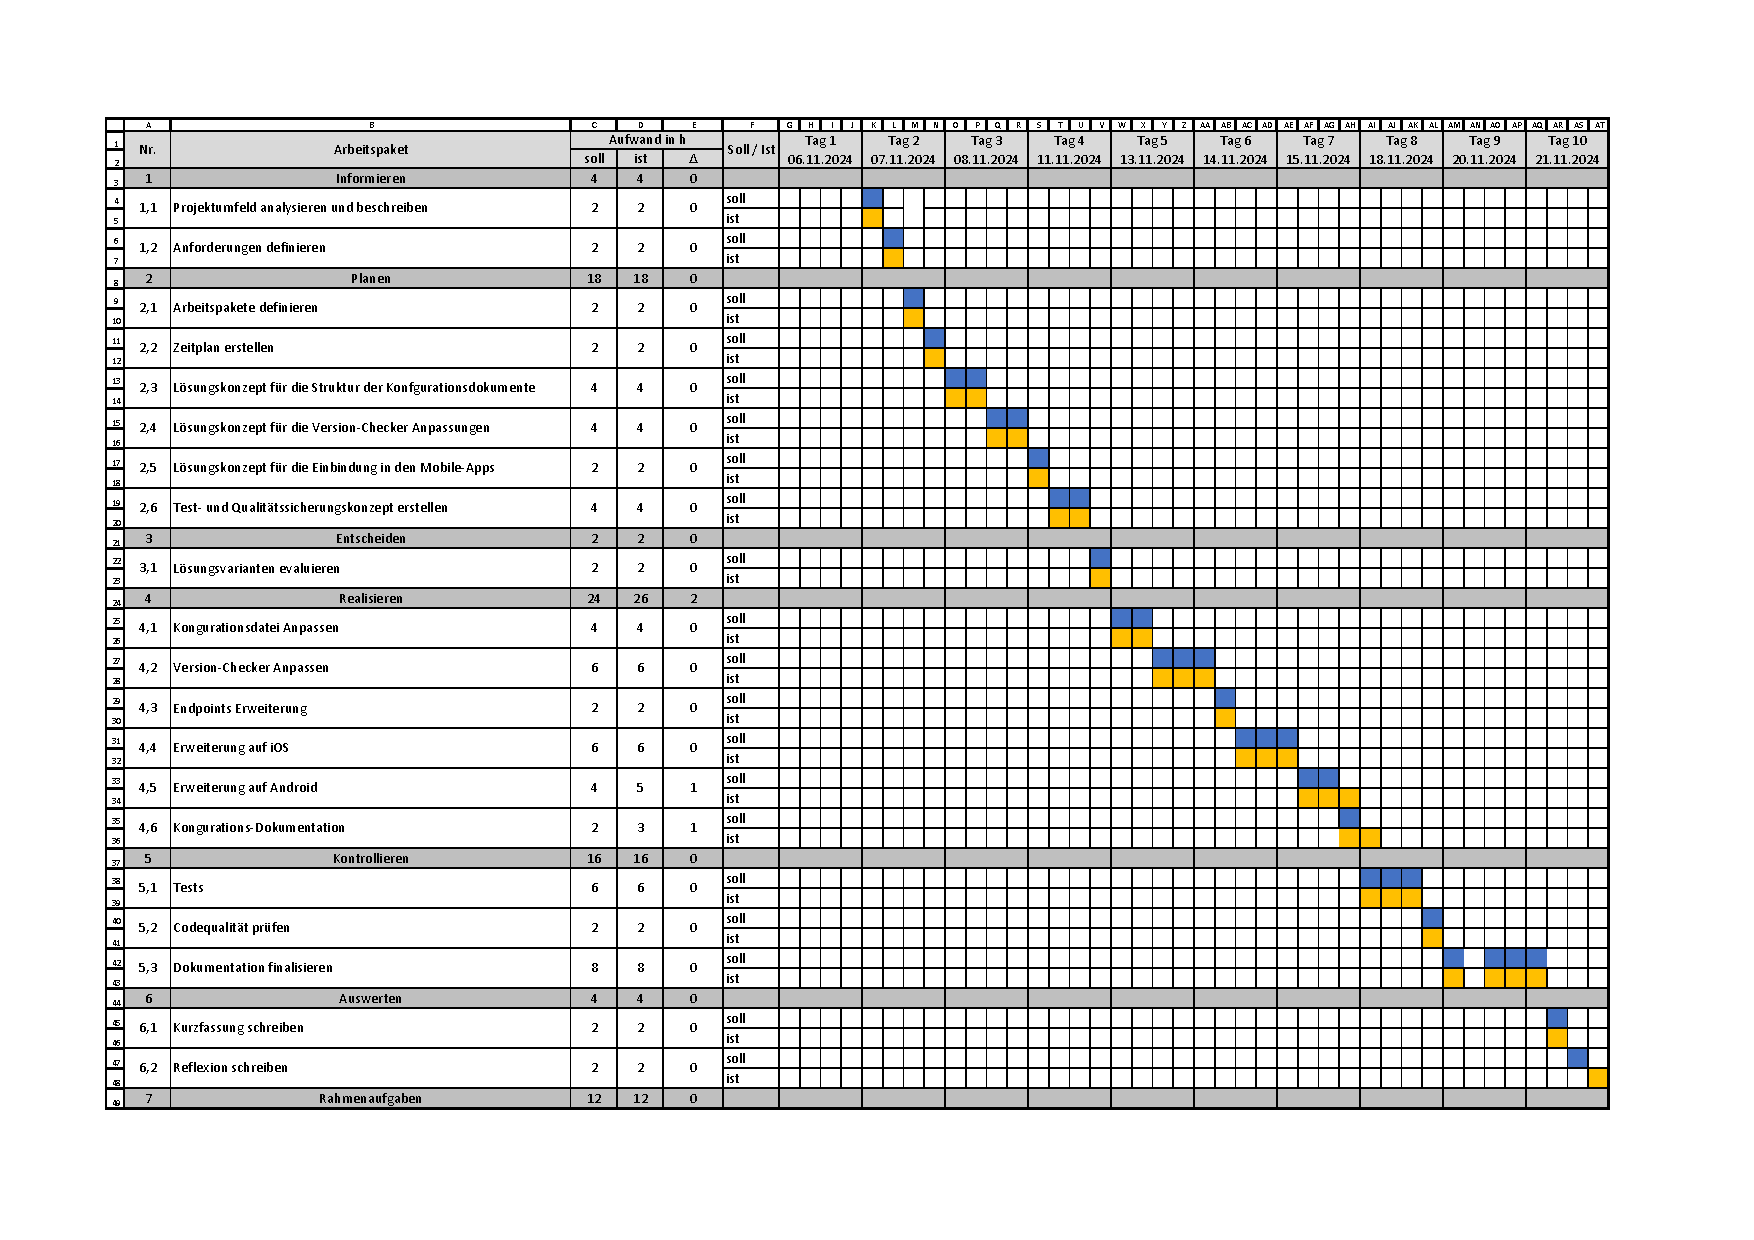
\includepdf[pages=-, angle=90]{ressourcen/zeitplan}
\end{landscape}



    \part{Projekt}\label{part:2}

    % Projekt Kapitel
	\chapter{Informieren}\label{ch:informieren}

In diesem Kapitel geht es um die erste von 6 Phasen der IPERKA-Methode, dem Informieren. Es bietet Platz um aufzuzeigen, was während dieser Phase unternommen wurde.

\section{Analyse}
Als erster Schritt wurde die Aufgabe analysiert, einen Überblick verschaffen und in folgender Kurzfassung zusammengefasst:
\subsection*{Kurzfassung}
Umzusetzen ist eine Funktion in der Admin App der Airlock IAM Applikation, welche es den Adminnuztern ermöglicht, die 16 stelligen Airlock 2FA Aktivierungscodes der Nutzer anzeigen zu lassen. Dies hilft Ihnen, die Endnutzer bei der Aktivierung der Airlock 2FA zu unterstützen. Der Aktivierungscode sollte per Konpfdruck angezeigt werden können, zum Beispiel als Popup. Dies ist jedoch noch zu evaluieren, vieleicht bieten sich auch noch andere Optionen an. Sicher ist, dass der Code im Airlock 2FA Management angezeigt werden soll und nur, falls durch den Admin gewollt. \newline
Weiter soll es mögllich sein, dass nicht alle Admins sich den Code anzeigen können, sondern nur die mit der entsprechenden Rollen. \newline
Das ganze muss mit UI, Unit und Integration Tests getestet werden, und in der Kundendokumentation ergänzt werden.

\subsection*{Abgrenzug}
Es gibt bereits die Funktionalität, dass Admins pro Nutzer Aktivierungsbriefe generieren können. Im Rahmen dieses Auftrags, soll dieser Bereich nicht erweitert oder verändert werden.

\subsection{Futurae}
Die Airlock 2FA App wird von Futurae entwickelt. Das hat zur Folge das zwischen IAM und Futurae wichtige Informationen ausgetauscht werden müssen. Dafür bietet Futurae 3 verschiedene API's an: die Auth API, die Admin API und die Log API. Für die Probe-IPA ist sowohl die Admin-API als auch die Auth-API relevant. Bei der Anfrage für den 16-stelligen Aktivierungscode wird zwar die Admin-API gebraucht, allerdings um den Code bei dem Start-Enrollment-Request zu erzwingen, wird auch die Auth-API verwendet werden müssen. Denn, Aktivierungen aus dem Protected so wie Public Self-Service führen über Auth-API. 

\section{Technische Referenzen}
Für die Techinschen Infos sind folgende zwei Links sehr hilfreich:
\begin{itemize}
	\item Futurae API: \url{https://www.futurae.com/docs/api/auth/}\newline
	 Da der Aktivierungs Code von Futurea kommt, ist dessen API Dokumentation eine wichtige Quelle.
	\item IAM Kunden Dokumentation: \url{https://docs.airlock.com/iam/8.3/}´
	Notwendig, um allgemeine Informationen bezüglich Airlock 2FA nachzulesen
\end{itemize}

\section{Anforderungen}
Nach der Analyse und nachdem der Auftrag verstanden wurde, konnten die Anforderungen definiert werden. Diese sind immer in funktionale und nicht-funktionale aufgeteilt.

Folgende Abkürzungen werden verwendet:
\begin{itemize}
	\item FA <Zahl> ... bedeutet funktionale Anforderung, mit nummerisch aufsteigendem Index.
	\item NFA <Zahl> ... bedeutet nicht-funktionale Anforderung, mit nummerisch aufsteigendem Index.
\end{itemize}

\subsection{Rest / Backend} \label{subsec:anforderungenBackend}

Folgend, sind die Anforderungen für das Backend resp. den Rest-Teil definiert.

\subsection*{Funktionale Anforderungen}
\begin{itemize}
	\item FA 1: Das Backend soll der SPA den Activation Code anbieten.
	\item FA 2: Der Activation Code darf nur angeboten werden, wenn der Admin auch die notwendige Rolle hat.
	\item FA 3: Im User Activities Logfile, soll geloggt werden, welcher Administrator zu welchem Zeitpunkt den 16-stelligen Aktivierungscode angezeigt hat.
	\item FA 4: Neue Plugins oder Properties sollen einen klaren und vollständigen Hilfetext haben.
\end{itemize}

\subsection*{Nicht-funktionale Anforderungen}
\begin{itemize}
	\item NFA 1: Sämtliche Fehlerfälle werden korrekt behandelt.
	\item NFA 2: Der Code entspricht dem bestehenden Codeschema.
	\item NFA 3: Alle neuen Funktionalitäten werden durch Tests abgedeckt.
	\item NFA 4: Veränderte / neue Restendpoints werden um die notwendige Doku erweitert.
\end{itemize}

\subsection{SPA} \label{subsec:anforderungenSPA}

Folgend, sind die Anforderungen für die SPA definiert.

\subsection*{Funktionale Anforderungen}
\begin{itemize}
	\item FA 5: Die SPA muss in der Lage sein den 16-stelligen QR-Code auf Knopfdruck anzuzeigen.
	\item FA 6: Das neue UI gleicht sich dem bisherigen Verhalten der SPA an.
	\item FA 7: Das neue UI hat den gleichen Style wie das bisherige.
	\item FA 8: Die Aktion, um den 16-stelligen Aktivierungscode anzuzeigen, sollte nur verfügbar sein, falls der Admin die nötigen Rollen hat, und ein offener Aktivierungscode existiert.
\end{itemize}

\subsection*{Nicht-funktionale Anforderungen}
\begin{itemize}
	\item NFA 5: Es werden nur in der Adminapp existierende UI Komponenten verwendet.
	\item NFA 6: Das UI lädt in jedem Fall ohne Probleme.
	\item NFA 7: Alle neuen Funktionalitäten werden durch Selenium Integration Tests abgedeckt.
\end{itemize}

\subsection{Kundendokumentation}

Folgend, sind die Anforderungen für die Kundendokumentation definiert.

\subsection*{Funktionale Anforderungen}
\begin{itemize}
	\item FA 9: Die Kunden Doku wird sinnvoll um das neue Feature erweitert.
	\item FA 10: Die Kundendoku ist auf Englisch geschrieben.
\end{itemize}

\subsection*{Nicht-funktionale Anforderungen}
\begin{itemize}
	\item NFA 8: Die Kundendoku hat keine Schreibfehler. 
	\item NFA 9: Die Kundendoku passt in das bestehende Produkt.
\end{itemize}
	\chapter{Planen}\label{ch:planen}
In diesem Abschnitt, wird die Planung beschrieben. In dieser Phase werden basierend auf den Anforderungen Arbeitspakete erstellt, und in einem GANT-Diagramm auf die 10 Tage eingeteilt.

\section{Arbeitspakete}

Um den ganzen Auftrag in kleine übersichtliche Teile aufzuteilen, wird er in verschiedene kleine Arbeitspakete unterteilt. Die Arbeitspakete sind jeweils nummeriert, haben einen Namen, einen geschätzten Aufwand in h und eine \flqq Definition of Done\frqq{}/ ein erwartetes Ergebnis. Die Aufwände sind oft mit einem gewissen Puffer geschätzt.\\
Die Pakete  sind nach den 6 Phasen der IPERKA Methode aufgelistet. Arbeiten welche IPA-spezifisch sind, sind unter Rahmenaufgaben aufgeführt.

\subsection{Informieren}
Hier, sind die Arbeitspakete, welche während der IPERKA-Phase \flqq Informieren\frqq{}\space bearbeitet wurden, aufgelistet.

\begin{longtable}{p{.22\textwidth}|p{.78\textwidth}}
	\hline
	\textbf{Nummer}    				& 1.1 \\
	\hline
	\textbf{Name}   				& Projektumfeld analysieren und beschreiben \\
	\hline
	\textbf{Geschätzter Aufwand}	& 2h \\
	\hline
	\textbf{Erwartetes Ergebnis}	& Das Ziel der Arbeit ist klar, ein grober Überblick besteht. \\
	\hline
\end{longtable}

\begin{longtable}{p{.22\textwidth}|p{.78\textwidth}}
	\hline
	\textbf{Nummer}    				& 1.2 \\
	\hline
	\textbf{Name}   				& Anforderungen definieren \\
	\hline
	\textbf{Geschätzter Aufwand}	& 2h \\
	\hline
	\textbf{Erwartetes Ergebnis}	& Die funktionalen und nicht-funktionalen Anforderungen sind definiert und beschrieben.\\
	\hline
\end{longtable}\pagebreak

\subsection{Planen}
Hier, sind die Arbeitspakete, welche während der IPERKA-Phase \flqq Planen\frqq{}\space bearbeitet werden, aufgelistet.

\begin{longtable}{p{.22\textwidth}|p{.78\textwidth}}
	\hline
	\textbf{Nummer}    				& 2.1 \\
	\hline
	\textbf{Name}   				& Arbeitspakete definieren \\
	\hline
	\textbf{Geschätzter Aufwand}	& 3h \\
	\hline
	\textbf{Erwartetes Ergebnis}	& Die ganze Arbeit ist in kleine logische Arbeitspakete unterteilt. Alle Arbeitspakete sind klar definiert.\\
	\hline
\end{longtable}

\begin{longtable}{p{.22\textwidth}|p{.78\textwidth}}
	\hline
	\textbf{Nummer}    				& 2.2 \\
	\hline
	\textbf{Name}   				& Zeitplan erstellen \\
	\hline
	\textbf{Geschätzter Aufwand}	& 1h \\
	\hline
	\textbf{Erwartetes Ergebnis}	& Der GANT-Zeitplan ist anhand der Arbeitspakete erstellt. Es sind alle Arbeitspakete vorhanden.\\
	\hline
\end{longtable}

\begin{longtable}{p{.22\textwidth}|p{.78\textwidth}}
	\hline
	\textbf{Nummer}    				& 2.3 \\
	\hline
	\textbf{Name}   				& Lösungskonzept für das Backend erarbeiten\\
	\hline
	\textbf{Geschätzter Aufwand}	& 4h \\
	\hline
	\textbf{Erwartetes Ergebnis}	& Es ist mindestens ein Lösungsvorschlag definiert und so weit wie Sinnvoll beschrieben und durchgedacht. Der relevante Backendcode ist verstanden.\\
	\hline
\end{longtable}\pagebreak

\begin{longtable}{p{.22\textwidth}|p{.78\textwidth}}
	\hline
	\textbf{Nummer}    				& 2.4 \\
	\hline
	\textbf{Name}   				& Lösungskonzept für die SPA erarbeiten\\
	\hline
	\textbf{Geschätzter Aufwand}	& 4h \\
	\hline
	\textbf{Erwartetes Ergebnis}	& Es ist mindestens ein Lösungsvorschlag definiert und so weit wie Sinnvoll beschrieben und durchgedacht. Es sind verschiedene Mockups vorhanden, und der relevante SPA Code ist verstanden.\\
	\hline
\end{longtable}

\begin{longtable}{p{.22\textwidth}|p{.78\textwidth}}
	\hline
	\textbf{Nummer}    				& 2.5 \\
	\hline
	\textbf{Name}   				& Test- und Qualitätssicherungskonzept erstellen\\
	\hline
	\textbf{Geschätzter Aufwand}	& 4h \\
	\hline
	\textbf{Erwartetes Ergebnis}	& Das Testkonzept ist erstellt und dokumentiert. Das Qualitätssicherungskonzept ist erstellt und dokumentiert.\\
	\hline
\end{longtable}

\subsection{Entscheiden}
Hier, sind die Arbeitspakete, welche während der IPERKA-Phase \flqq Entscheiden\frqq{}\space bearbeitet werden, aufgelistet.

\begin{longtable}{p{.22\textwidth}|p{.78\textwidth}}
	\hline
	\textbf{Nummer}    				& 3.1 \\
	\hline
	\textbf{Name}   				& Lösungsvarianten evaluieren \\
	\hline
	\textbf{Geschätzter Aufwand}	& 2h \\
	\hline
	\textbf{Erwartetes Ergebnis}	& Aus den verschiedenen Lösungsvarianten der SPA und des Backends wurde sich für eine entschieden, und dies Dokumentiert.\\
	\hline
\end{longtable}\pagebreak

\subsection{Realisieren}
Hier, sind die Arbeitspakete, welche während der IPERKA-Phase \flqq Realisieren\frqq{}\space bearbeitet werden, aufgelistet.

\begin{longtable}{p{.22\textwidth}|p{.78\textwidth}}
	\hline
	\textbf{Nummer}    				& 4.1 \\
	\hline
	\textbf{Name}   				& Das Backend erweitern  \\
	\hline
	\textbf{Geschätzter Aufwand}	& 14h \\
	\hline
	\textbf{Erwartetes Ergebnis}	& Alle Anforderungen für das Backend sind nach dem definierten Lösungsansatz umgesetzt. Zugleich ist die Lösung dokumentiert. \\
	\hline
\end{longtable}

\begin{longtable}{p{.22\textwidth}|p{.78\textwidth}}
	\hline
	\textbf{Nummer}    				& 4.2 \\
	\hline
	\textbf{Name}   				& Unit- und Integrationtests schreiben  \\
	\hline
	\textbf{Geschätzter Aufwand}	& 6h \\
	\hline
	\textbf{Erwartetes Ergebnis}	& Alle neuen Funktionalitäten sind mit Unit- und/oder Integrationtests getestet.\\
	\hline
\end{longtable}


\begin{longtable}{p{.22\textwidth}|p{.78\textwidth}}
	\hline
	\textbf{Nummer}    				& 4.3 \\
	\hline
	\textbf{Name}   				& Die SPA erweitern  \\
	\hline
	\textbf{Geschätzter Aufwand}	& 6h \\
	\hline
	\textbf{Erwartetes Ergebnis}	& Alle Anforderungen für die SPA sind nach dem definierten Lösungsansatz umgesetzt. Zugleich ist die Lösung dokumentiert.\\
	\hline
\end{longtable}

\begin{longtable}{p{.22\textwidth}|p{.78\textwidth}}
	\hline
	\textbf{Nummer}    				& 4.4 \\
	\hline
	\textbf{Name}   				& Selenium Integrationtests implementieren  \\
	\hline
	\textbf{Geschätzter Aufwand}	& 5h \\
	\hline
	\textbf{Erwartetes Ergebnis}	& Alle neuen Funktionalitäten sind mit Selenium Integrationtests getestet.\\
	\hline
\end{longtable}\pagebreak

\begin{longtable}{p{.22\textwidth}|p{.78\textwidth}}
	\hline
	\textbf{Nummer}    				& 4.5 \\
	\hline
	\textbf{Name}   				& Kundendokumentation schreiben  \\
	\hline
	\textbf{Geschätzter Aufwand}	& 2h \\
	\hline
	\textbf{Erwartetes Ergebnis}	& Die neue Funktionalität ist in der Kundendokumentation dokumentiert, und alle Anforderungen sind erfüllt.\\
	\hline
\end{longtable}


\subsection{Kontrollieren}
Hier, sind die Arbeitspakete, welche während der IPERKA-Phase \flqq Kontrollieren\frqq{}\space bearbeitet werden, aufgelistet.

\begin{longtable}{p{.22\textwidth}|p{.78\textwidth}}
	\hline
	\textbf{Nummer}    				& 5.1 \\
	\hline
	\textbf{Name}   				& Tests durchführen, und Fehler beheben \\
	\hline
	\textbf{Geschätzter Aufwand}	& 4h
	h \\
	\hline
	\textbf{Erwartetes Ergebnis}	& Tests sind gemäss Testkonzept durchgeführt, und mögliche Fehler sind behoben. \\
	\hline
\end{longtable}

\begin{longtable}{p{.22\textwidth}|p{.78\textwidth}}
	\hline
	\textbf{Nummer}    				& 5.2 \\
	\hline
	\textbf{Name}   				& Codequalität prüfen, und Refactorn \\
	\hline
	\textbf{Geschätzter Aufwand}	& 1h \\
	\hline
	\textbf{Erwartetes Ergebnis}	& Code ist nochmals durchgeschaut, und Unschönheiten sind bereinigt.\\
	\hline
\end{longtable}

\begin{longtable}{p{.22\textwidth}|p{.78\textwidth}}
	\hline
	\textbf{Nummer}    				& 5.3 \\
	\hline
	\textbf{Name}   				& Dokumentation finalisieren \\
	\hline
	\textbf{Geschätzter Aufwand}	& 8h \\
	\hline
	\textbf{Erwartetes Ergebnis}	& Die Dokumentation ist soweit wie möglich finalisiert und entspricht den Vorgaben.\\
	\hline
\end{longtable}

\subsection{Auswerten}
Hier, sind die Arbeitspakete, welche während der letzten IPERKA-Phase \flqq Auswerten\frqq{}\space bearbeitet werden, aufgelistet.

\begin{longtable}{p{.22\textwidth}|p{.78\textwidth}}
	\hline
	\textbf{Nummer}    				& 6.2 \\
	\hline
	\textbf{Name}   				& Reflexion schreiben \\
	\hline
	\textbf{Geschätzter Aufwand}	& 2h \\
	\hline
	\textbf{Erwartetes Ergebnis}	& Reflexion zu den relevanten Abschnitten ist geschrieben. \\
	\hline
\end{longtable}

\subsection{Rahmenaufgaben}
Hier, sind die Arbeitspakete, welche IPA-spezifische Arbeit erfordern, aufgelistet.

\begin{longtable}{p{.22\textwidth}|p{.78\textwidth}}
	\hline
	\textbf{Nummer}    				& 7.1 \\
	\hline
	\textbf{Name}   				& Projektstruktur aufsetzen\\
	\hline
	\textbf{Geschätzter Aufwand}	& 2h \\
	\hline
	\textbf{Erwartetes Ergebnis}	& Das Grundgerüst für den Bericht steht. Der Latex-Build ist lauffähig und generiert ein anschaubares PDF.\\
	\hline
\end{longtable}

\begin{longtable}{p{.22\textwidth}|p{.78\textwidth}}
	\hline
	\textbf{Nummer}    				& 7.2 \\
	\hline
	\textbf{Name}   				& Aufgabenstellung und Rahmenbedingungen beschreiben\\
	\hline
	\textbf{Geschätzter Aufwand}	& 1h \\
	\hline
	\textbf{Erwartetes Ergebnis}	& Die Aufgabenstellung ist in den Bericht übernommen. Benützte Firmenstandarts sowie die Projektaufbauorganisation sind defniert und beschrieben. \\
	\hline
\end{longtable}

\newpage

\begin{longtable}{p{.22\textwidth}|p{.78\textwidth}}
	\hline
	\textbf{Nummer}    				& 7.3 \\
	\hline
	\textbf{Name}   				& Projektmanagementmethode definieren\\
	\hline
	\textbf{Geschätzter Aufwand}	& 1h \\
	\hline
	\textbf{Erwartetes Ergebnis}	& Es steht fest mit welcher Projektmanagementmethode die Probe-IPA umgesetzt werden soll. Der Bericht wurde so gegliedert.\\
	\hline
\end{longtable}

\begin{longtable}{p{.22\textwidth}|p{.78\textwidth}}
	\hline
	\textbf{Nummer}    				& 7.4 \\
	\hline
	\textbf{Name}   				& Expertenbesuche\\
	\hline
	\textbf{Geschätzter Aufwand}	& 4h \\
	\hline
	\textbf{Erwartetes Ergebnis}	& Infos aus dem Gespräch sind am richtigen Ort festgehalten.\\
	\hline
\end{longtable}

\begin{longtable}{p{.22\textwidth}|p{.78\textwidth}}
	\hline
	\textbf{Nummer}    				& 7.5 \\
	\hline
	\textbf{Name}   				& Anhang erstellen\\
	\hline
	\textbf{Geschätzter Aufwand}	& 2h \\
	\hline
	\textbf{Erwartetes Ergebnis}	& Der Anhang ist erstellt und beinhaltet alle nötigen und verlangten Inhalte.\\
	\hline
\end{longtable} 
\newpage

\section{Lösungskonzept Backend}

In diesem Kapitel ist das Lösungskonzept für das Backend beschrieben. Das Konzept richtet sich nach den in Kapitel \ref{subsec:anforderungenBackend} definierten Anforderungen. Es wurden diverse TODO's im Code hinzugefügt, dies macht die Implementation danach viel effizienter.

\subsection{REST}\label{subsec:rest}

Damit die SPA den 16-stelligen Aktivierungscode anzeigen kann, muss er mit Hilfe einer REST-Schnittstelle übermittelt werden. Dass er aber überhaupt von Futurae erstellt wird, muss er bei dem Enrollement, also dem Call der einen neuen Nutzer erstellt, explizit gefordert werden. 
Dies funktioniert in dem man den Requestparameter \flqq short\_code\frqq{} auf true setzt. Für die Übermittlung an die SPA stehen 2 Optionen im Raum:

\begin{itemize}
	\item Option 1: Den Endpunkt, welcher alle Accountdaten von jedem Nutzer zurück gibt um den Activation Code erweitern. Dies hätte zur Folge das der Endpunkt um ein optionales Feld \flqq activation\_code\_short\frqq{}\space erweitert wird.
	\label{"itm:restOption1"}
	\item Option 2: Einen neuen Endpunkt erstellen, welcher den offenen Aktivierungscode zurück gibt. Dies wäre ein einfacher GET-Endpunkte, welcher, falls vorhanden den neusten, austehenden Aktivierungscode zurück gibt. Folgend eine kurze Spezifikation des Endpunktes:\\\\

	\textbf{Pfad:} /auth-admin/rest/users/{userId}/tokens/airlock-2fa/activation-code-short\\
	\textbf{HTTP-Methode:} GET\\
	\textbf{Pfadparameter:} userid\\
	\textbf{Response:} Optionaler Actiovation Code, kann leer sein \newline
	\textbf{Status Codes:}
	\begin{longtable}{p{.25\textwidth}|p{.55\textwidth}}
		\hline
		\textbf{200 Ok}    				& 16-stelliger Aktivierungscode oder nichts \\
		\hline
		\textbf{401 Unauthorized}   				& Invalide oder fehlende Authentifizierung\\
		\hline
		\textbf{403 Forbidden}	& Der Zugriff ist verboten (z.B fehlende Adminrolle) \\
		\hline
		\textbf{404 Not Found}	& Mögliche Error Codes:
		\begin{itemize}
			\item USER\_NOT\_FOUND 
			\item ACCOUNT\_NOT\_FOUND
		\end{itemize}\\
		\hline
	\end{longtable} 
	
	\label{"itm:restOption2"}	
\end{itemize}

In beiden Fällen müsste der Restflow so aussehen:
\begin{figure}[H]
	\begin{center}
		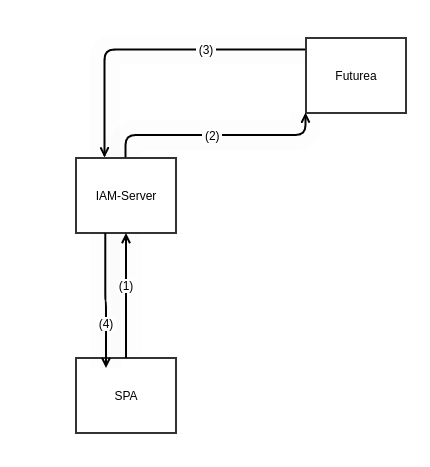
\includegraphics[width=0.8\textwidth]{ressourcen/restflow}
		\caption[Restflow]{Restflow um 16-stelligen Aktivierungscode zu bekommen}\label{fig:restflow}
	\end{center}
\end{figure}

\begin{itemize}
	\item[(1)] Die SPA macht als Reaktion auf einen Klick einen Request, ans IAM Backend. Je nach Option, geht dieser an einen anderen Endpunkt. 
	\item[(2)] Das Backend macht folgenden Request an Futurae: \newline
	/srv/admin/v1/enrollments?status=pending
	\item[(3)] 	Da bei dem Enrollment Request zu Futurae der 16-stellige Aktivierungscode explizit gefordert wurde, wird dieser Request, falls überhaupt ein austehendes Enrollment vorhanden ist, dieses auch zurück geben. Da mehere offene Enrollments vorhanden sein können, muss immer das Neuste genommen werden. Damit immer klar ist welcher Code zurück kommt. Helpdesk oder Schalter Mitarbeiter können so die Aktivierung direkt mit dem Kunden durchspielen.
	\item[(4)] Das Backend gibt den Aktivierungscode an die SPA weiter. Je nach Option auch noch die anderen Accountdaten. Falls keiner vorhanden ist, wird die Response einfach leer gelassen, resp. das Feld.
\end{itemize}


\subsection{Rollenlogik}
Es gibt bereits eine Regel, welche das Ansehen von Aktivierungsdaten einschränkt. Diese Regel kann wiederverwendet werden. Dazu gibt es einen \flqq Airlock2FAAccessController.java.\frqq{} Dieser kann beim erstellen der Response injected werden. Mit der Methode \flqq isAllowedToSeeActivationSecrets\frqq{} \space kann dann überprüft werden, ob der Adminnutzer diese Info überhaupt sehen darf. Am besten wird dieser Check noch vor dem Futurae Request ausgführt, um einen unnötigen Rountrip zu vermeiden und es möglichst effizient zu halten. Falls die Option mit einem neuen Endpunkt gewählt wird, kann dieser separat protected werden, dann fällt die Logik weg.

\subsection{Wichtige Klassen und Interfaces}
\textbf{Option 1}
\begin{itemize}
	\item UserAirlock2FADeviceResource.java: In dieser Klasse befindet sich der Endpoint \flqq /auth-admin/rest/users/{userId}/tokens/airlock-2fa \frqq{}, welcher erweitert werden könnte. 
	\item Airlock2FAUserAccount.java dies ist die Klasse welche die wichtigen Daten über den Acount beinhaltet. Diese Klasse muss um das Feld \flqq activationCodeShort\frqq{} erweitert werden.
	\item Airlock2FAAdminService.java: Dieser Service wird aus der Resource aufgerufen, um den Account von der Datenbank zu bekommen.
	\item Airlock2FAUserAccountRepository.java: Das Repository ist die Schnittstelle zwischen der Datenbank und dem Service. Die darin enthaltene \flqq findBy()\frqq{} Methode gibt schluss endlich den zusammengestellten \flqq Airlock2FAUserAccount.java\frqq{} zurück.
\end{itemize}
\textbf{Option 2}
\begin{itemize}
	\item UserAirlock2FADeviceResource.java: In dieser Klasse wird der oben definierte Endpunkt \flqq /auth-admin/rest/users/{userId}/tokens/airlock-2fa/activation-code-short \frqq{} erstellt.
\end{itemize}
\textbf{Request zu Futurae}\newline
Der Request zu Futurae wird in beiden Optionen gleich aussehen. Lediglich der \flqq FuturaeAdminApiEnrollmentServiceImpl.java\frqq{} wird an verschiedenen Orten gebraucht.
\begin{itemize}
	\item FuturaeAdminApiEnrollmentServiceImpl.java: In diesem Serivce muss der\\ Airlock2FAAccessController injected werden. Zusätzlich wird es eine neue Methode geben müssen, welche zuerst mit Hilfe des Airlock2FAAccessController prüft, ob der Adminnutzer die richtige Rolle hat. Danach wird via die \flqq FuturaeAdminApiEnrollmentRequestFactory.java\frqq{} der Request zusammengestellt. Dieser Request wird dann via den RestClient ausgeführt. Die Response wird dann in ein neu erstelltes ...Response Objekt gespeichert und zurück gegeben.
	\item FuturaeAdminApiEnrollmentRequestFactory.java: In dieser Klasse braucht es eine neue Methode welche einen Request zusammenstellt, der von Futurae die neueste offene Aktivierung anfragt.
	\item AdminEnrollmentRequest.java: Diese Klasse bildet den Admin Request ab, welcher gesendet wird um neue Geräte zu aktivieren. Er muss um das Feld \flqq short\_code\frqq{} erweitert werden. Dieses Feld muss anschliessend auf true gestzt werden.
	\item FuturaeAuthApiEnrollmentRequestFactory.java: Es ist wichtig auch in dieser Klasse auf dem Enrollmentrequest \flqq short\_code\frqq{} auf true zu setzen, ansonsten wird der 16-stellige Aktivierungscode nicht erzwungen, wenn das Enrollment von einem Endnutzer aus dem Self-Service gestartet wrid. Denn dann verläuft es über die Auth API. 
\end{itemize}



\section{Lösungskonzept SPA}\label{sec:lk-spa}
In diesem Kapitel werden die Lösungsideen für das Frontend / die SPA dokumentiert.  Das Konzept richtet sich nach den in Kapitel \ref{subsec:anforderungenSPA} definierten Anforderungen. Es wurden diverse TODO's im Code hinzugefügt, dies macht die Implementation danach viel effizienter. 

\subsection{Mockups}
Um sich eine Vorstellung zu machen, wurden zuerst verschiedene Mockups erstellt. Da es fürs UI keine grosse Änderung ist, konnten die Mockups grössten Teils direkt im Code erstellt werden, natürlich ohne funktionalität. \newline\\
Auf dem folgende Bild ist die Adminapp im Airlock 2FA Mangement des Nutzers \flqq itester\frqq{}. Es wird davon ausgegangen das der Admin die nötigen Rollen hat, um sich den Aktivierungscode anzuzeigen. 
\begin{figure}[H]
	\begin{center}
		\caption[UI Mockup]{Das folgende Bild zeigt den UI Vorschlag}\label{fig:mockup1}
	\end{center}
\end{figure}
\begin{landscape}
	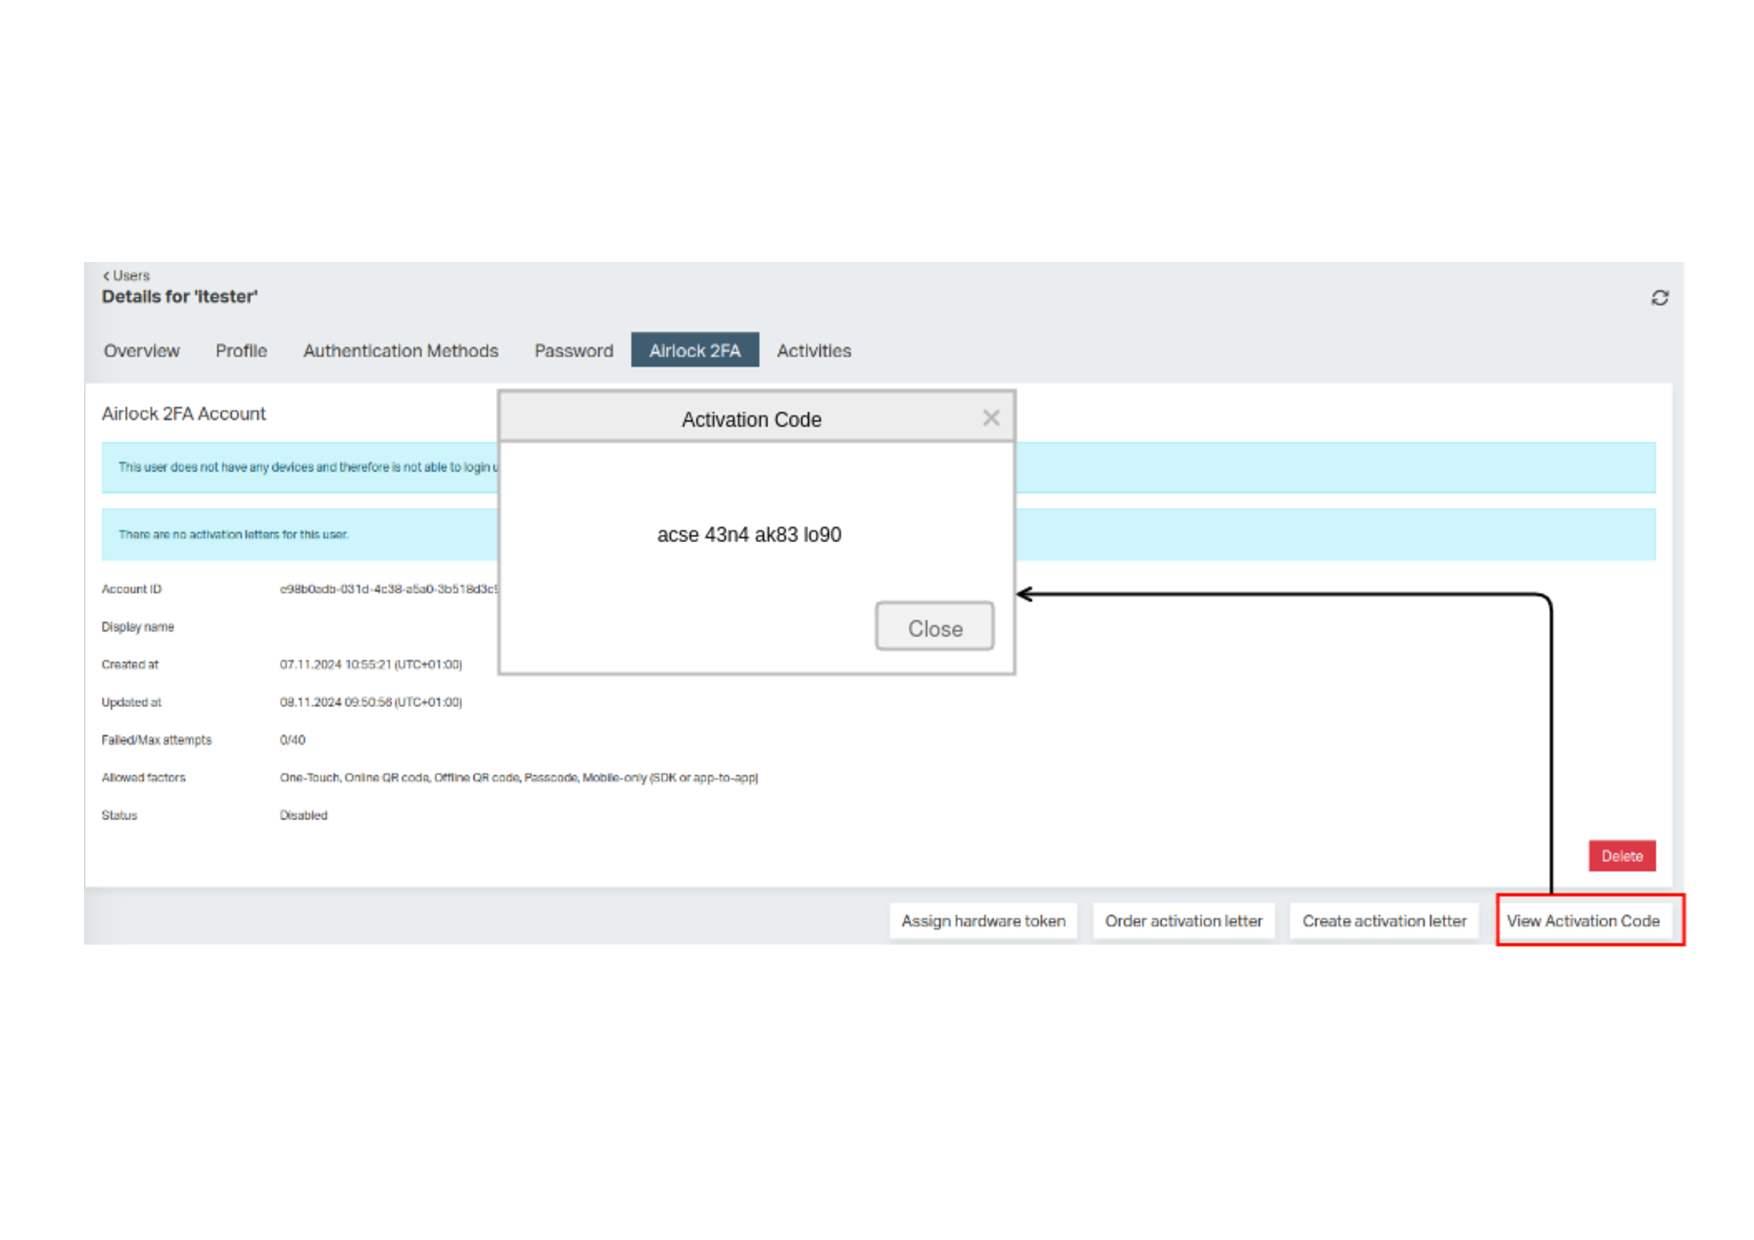
\includepdf[pages=-, angle=90]{ressourcen/Mockup1}
\end{landscape}
\noindent Es der Ansatz verfolgt, dass unten rechts ein weiterer Button hinzukommt. Dieser wird allerdings nur dann angezeigt, wenn der Admin auch die nötigen Rollen dazu hat und ein offener Aktivierungscode vorhanden ist(sprich nicht null zurück kommt). Wird der Button geklickt, soll sich ein Popup öffnen, in dem der 16-stellige Aktivierungscode angezeigt wird. Ev. könnte es auch eine Option sein, das Enrollmentdatum auch noch anzuzeigen, das könnte bei Fehlversuchen dem Admin eventuell hilfreich sein. Dies könnte dann in etwa so aussehen:
\begin{figure}[H]
	\begin{center}
		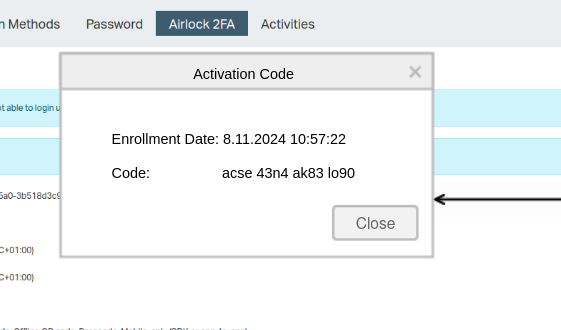
\includegraphics[width=0.8\textwidth]{ressourcen/popup}
		\caption[Popup mit Datum]{Popup Variante mit Datum}\label{fig:restflow}
	\end{center}
\end{figure}

\subsection{Lösungsvariante ohne Popup}
Anstelle eines Popups, welches durch einen Button ausgelöst wird, könnte man in der Accountübersicht auch folgendes einbauen:
\begin{figure}[H]
	\begin{center}
		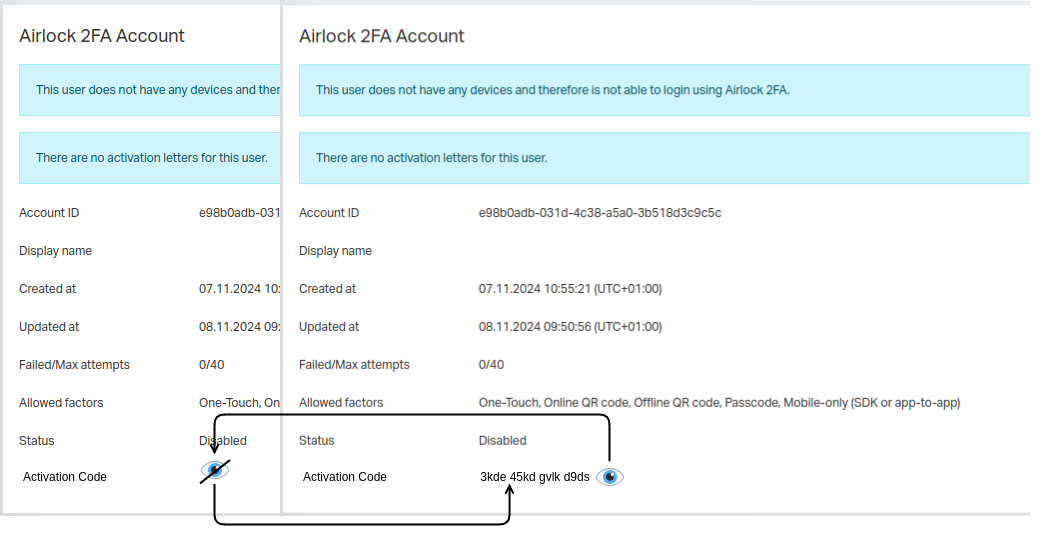
\includegraphics[width=1.0\textwidth]{ressourcen/variant_2_spa}
		\caption[Variante ohne Popup]{SPA Lösung ohne Popup}\label{fig:withoutpopup}
	\end{center}
\end{figure}
\noindent Analog zu einer Passwortanzeige könnte man es mit einem Auge darstellen. Wird auf das durchgestrichene Auge geklickt wird der Code angezeigt. Wird dann wieder auf das offene Auge geklickt, verschwindet der Aktivierungscode wieder.\newline
Diese neue Zeile wird nur dann angezeigt, wenn auch ein Aktivierungscode vorhanden ist und der Admin die erforderlichen Rechte hat.

\subsection{Rollenlogik}
Damit sichergestellt wird, dass der Button nur dann angezeigt wird, wenn der Benutzer dies möchte, kann ihm das Attribut \flqq hideOnAccessDenied\frqq{} gesetzt werden. Der Button braucht zudem ein sprechende ID. Diese ID wird dann im Access Controller im Backend, als Permissonkey verwendet.

\subsection{Wichtige Komponenten und Services}
\begin{itemize}
	\item airlock-2fa.component.html: In diesem File wird die Darstellung des UI definiert. Hier muss der neue Button hinzugefügt werden.
	\item airlock-2fa.service.ts: In diesem Service wird der Request an das IAM-Backend gemacht, um den Aktivierungscode zu bekommen. Anschliessend wird sie geparsed und zurückgegeben.
	\item airlock-2fa.component.ts: In dieser Component, wird die Logik für den neuen Button implementiert. Konkret:
	\begin{itemize}
		\item Beim laden der Komponente wird via den obigen Service, der Aktivierungscode abgefragt.  
		\item Er darf nur angezeigt werden, falls auch ein Aktivierungs Code vorhanden ist.
		\item Wird er angecklickt, öffnet sich ein Popup mit dem aktuellsten, offenen, 16-stelligen Aktivierungscode.
	\end{itemize}
	\item Zudem wird es ein neues Model für den Aktivierungscode geben müssen, falls das Datum auch angezeigt werden soll. Das sollte wie folgt aussehen:
		\begin{lstlisting}[language=TypeScript]
export interface Airlock2FAActivationCodeData {
		activationCodeShort: string;
		enrollmentDate: Date;
}
		\end{lstlisting}
\end{itemize}
\subsection{Translation Keys}
Um in der Adminapp die Sprachen Deutsch, Englisch und Französisch zu unterstützen wird i18n verwendet. Dafür wird für jeden String in der SPA ein Translation Key definiert. Hierfür gibt es 3 verschiedene JSON-Files; für jede Sprache eines. Das Value ist, dann der übersetzte Text in die jeweilige Sprache. Je nach Sprache wird nun ein anderes JSON-File angezogen, dies führt dazu, dass immer die korrekte Übersetzung verwendet wird. In diesem Fall benötigt es mindestens folgende 2 Keys:
\begin{itemize}
	\item user.airlock-2fa.activation.view-activation-code.button: Text im Button
	\item user.airlock-2fa.activation.view-activation-code.popup.title: Titel des Popup's
	\item user.airlock-2fa.activation.view-activation-code.popup.text: Text im Popup
\end{itemize}

\section{Testkonzept} \label{sec:testkonzept}
Das neue Feature soll fehlerfrei und nach den Anforderungen funktionieren. Um dies Sicherzustellen wird folgend ein Testkonzept zusammen gestellt, nach welchem das Feature später getestet werden sollte.
Alle erwähnten Technologien sind in Kapitel \ref{sec:verwendete-tools} beschrieben.


\subsection{Benötigte Testmittel}
Unit-Tests und Integrations-Tests werden von der Entwicklungsumgebung Intellij ausgeführt. Da die Applikation lokal auch aus dem Intellij gestartet werden kann, werden auch die manuellen Tests mit der Hilfe von Intellij durchgeführt.  \newline
\\
Damit sichergegangen werden kann, dass nicht nur die neuen Funktionen funktionieren, sondern alles darum herum auch noch, führt Jenkins bei jedem Push eines neuen Patchsets alle Tests aus. Failed dieser Build, ist etwas kaputt.

\subsection{Wiremock} \label{subsec:wiremock}
In gewissen Unit- sowie allen Integration- Tests wird Wiremock verwendet um den Futurae Server zu simulieren. Wiremock stellt dabei einen Dummy-Server zurverfügung, das heisst alle Anfragen gehen an diesen Server und somit nicht über das Netzwerk. Dies verhindert Flaky Tests und bietet eine konstante und auf den Testcase angepasste API. 

\subsection{Unit-Tests}
Unit-Tests werden verwendet um die Kernlogik in kleinen isolierten Einheiten zu testen. Hierfür werden komplexe Umsysteme oder Klassen gemockt. Dies wird mit Mockito gemacht. Die Tests ansich werden mit JUnit5 implementiert. Konkret für diesen Auftrag müssen folgende Kernfunktionalitäten mit Unit-Tests abgedeckt werden:
\begin{itemize}
	\item Check, ob ein Admin die richtigen Rollen besitzt.
	\item Die neue Funktion im FuturaeAdminApiEnrollmentServiceImpl.java welche den neusten, offenen Aktivierungscode zurück gibt.	
\end{itemize}

\subsection{REST-Integration-Tests}
Die REST-Integration-Tests werden auch mit hilfe von JUnit geschrieben. Anderst als bei den Unit-Tests wird hier nicht eine kleine Einheit getestet sondern der ganze Teil von der Restresource bis zur Datenbank.
Mit den Integrationtests wird sicher gestellt, dass das ganze Feature im Backend richtig funktioniert. Für das sind folgende zwingende Fälle zu testen:

\begin{itemize}
	\item Es dürfen nur berechtigte Admins den Code erhalten.
	\item Es muss eine 403 Response zurück kommen, wenn ein Admin nicht berechtigt ist.
	\item Falls kein offenes Enrollment existiert, der Admin aber berechtigt wäre, muss die Response leer sein.
	\item Es muss geloggt werden, welcher Admin, sich wann, welchen Aktivierungscode, angeschaut hat.
\end{itemize}

\subsection{UI-Integration-Tests}
Zusätzlich zu den Rest-Integration-Tests werden auch UI-Integration-Tests erstellt. Diese Tests werden mit Selenium ausgeführt. Mit ihnen wird das UI / die SPA im Zusammenspiel mit dem IAM-Backend getestet.
Folgende fälle sind zu Testen:
\begin{itemize}
	\item Hat der Admin keine Berechtigung, darf der Button gar nicht erst angezeigt werden.
	\item Hat der Admin die Berechtigung, es gibt jedoch keinen Activation Code, darf der Button auch nicht angezeigt werden.
	\item Hat der Admin die Berechtigung und es ist ein Activation Code vorhanden, muss der Button angezeigt werden.
	\item Wird der Button geklickt wird ein Popup aufgehen, in welchem der Activation Code steht.
	\item Klickt man in diesem Popup auf Schliessen sollte man wieder auf der Airlock 2FA Mangamentseite landen.
\end{itemize}
\newpage

\subsection{Manuelle Tests} \label{subsec:mtests}
Die Funktionalitäten werden durch die vielen automatisierten Tests schon recht gut getestet. Allerdings ist es auch wichtig, das ganze manuell zu Testen. Der wichtigste Grund ist, dass der Futurae Server nicht mehr gemockt ist, sondern nun eine richtige Verbindung besteht. Damit es nicht zu unerwarteten Aktionen kommt, sind diese Test sehr wichtig. Für die manuellen Tests sind folgende Testfälle definiert:

	\begin{longtable}{p{.25\textwidth}|p{.55\textwidth}}
	\hline
	\textbf{Testfall}    			& M1 \\
	\hline
	\textbf{Testumgebung}	& 
	\begin{itemize}
		\item IAM auf Localhost 
		\item Demokonfiguration ergänzt mit der Konfiguration des Futurae Service.
	\end{itemize}\\
	\hline
	\textbf{Beschreibung}   		& Der Admin hat die nötigen Rollen, damit er den Aktivierungscode ansehen kann und es gibt ein Enrollment welches offen ist. Der Admin klickt auf den Button, welcher ihm den Aktivierungscode anzeigen soll. \\
	\hline
	\textbf{Erwartetes Resultat}	& Es öffnet sich ein Popup (kein Browserpupop), mit dem Aktivierungscode, und allenfalls dem Enrollmentdatum. \\
	\hline
	
\end{longtable} 
	\begin{longtable}{p{.25\textwidth}|p{.55\textwidth}}
	\hline
	\textbf{Testfall}    			& M2 \\
	\hline
	\textbf{Testumgebung}	& 
	\begin{itemize}
		\item IAM auf Localhost 
		\item Demokonfiguration ergänzt mit der Konfiguration des Futurae Service.
		\item Postman um Request ohne SPA abzusetzen
	\end{itemize}\\
	\hline
	\textbf{Beschreibung}   		& Der Admin hat die nötigen Rollen nicht, damit er den Aktivierungscode ansehen kann und es gibt ein Enrollment welches offen ist.\\
	\hline
	\textbf{Erwartetes Resultat}	& Der Button wird nicht angezeigt. Der Admin darf auch via Postman den Aktivierungscode nicht bekommen. \\
	\hline
	
\end{longtable} 
\newpage

\begin{longtable}{p{.25\textwidth}|p{.55\textwidth}}
\hline
\textbf{Testfall}    			& M3 \\
\hline
\textbf{Testumgebung}	& 
\begin{itemize}
	\item IAM auf Localhost 
	\item Demokonfiguration ergänzt mit der Konfiguration des Futurae Service.
\end{itemize}\\
\hline
\textbf{Beschreibung}   		& Der Admin hat die nötigen Rollen nicht, damit er den Aktivierungscode ansehen kann und es gibt kein Enrollment welches offen ist.\\
\hline
\textbf{Erwartetes Resultat}	& Der Button wird nicht angezeigt. \\
\hline

\end{longtable}  

\section{Qualitätssicherungskonzept}
Das Qualitätssicherungskonzept wird definiert, um eine möglichst hohe Qualität des Codes zu erhalten.
\newline
Die Qualität des Codes ist im IAM-Repository schon sehr gut erzwungen. Durch Architecture Layering Tests und Checkstyle sind IAM-Spezifische Vorgaben getestet, damit der Code einheitlich bleibt. Zusätzlich gibt es auch noch PMD und Spotbugs Checks. Die PMD Checks prüfen den Code auf unschönheiten, basierend auf IAM-spezifischen Regeln. Das selbe gilt für SpotBugs.
\newline
Durch all diese Tests wird die Qualität sehr gut sichergestellt. Bei jedem Push eines neuen Patchsets werden diese Checks, zusätzlich zu den normalen Tests, auch in der Jenkinspipeline ausgeführt.








	\chapter{Entscheiden}\label{ch:entscheiden}
Dieses Kapitel bietet Platz, für die IPERKA-Phase \flqq Entscheiden\frqq{}. Es werden die verschiedenen Vorschläge aus der Planungsphase zu evaluiert und sich für den besten Weg entschieden.
\section{REST-Interface Backend}
In Abschnitt \ref{subsec:rest} wurden folgende 2 Lösungsvarianten für die REST-Schnittstelle definiert:
\begin{itemize}
	\item{Option 1:} Den bestehenden Endpunk, welcher den Account des Nutzers zurück gibt um das Activationcode Feld erweitern.
	\item{Option 2:} Einen neuen separaten Endpunkt welcher nur den Activationcode, und eventuell noch weitere Daten wie das Enrollment Datum zurück gibt.
\end{itemize}
Die 2 Varianten werden basierend auf folgenden Eigenschaften verglichen:
\newline\\
\textbf{Flexibilität} Je flexibler der Activationcode angefragt werden kann desto besser. Dadurch kann er einfach durch weitere Infos ergänzt werden.\\\\
\textbf{Beachtung der Rollen} Zugriffskontrolle basierend auf den Rollen des Adminnutzers kann einfach eingeschränkt werden.
\\\\
\textbf{Aufwand} Der Aufwand sollte sich in Grenzen halten, da nur begrenzt Zeit vorhanden ist.
\\
\\
In der folgenden Nutzwertanalyse werden die beiden Varianten miteinander verglichen und jeweils mit 0-10 Punkten bewertet, welche mit der Gewichtung des Kriteriums multipliziert werden:
\begin{longtable}{|p{.22\textwidth}|p{.40\textwidth}|p{.38\textwidth}|}
	\hline
	\textbf{Kriterium und Gewichtung} & \textbf{Option 1 (Endpunk erweitern)} & \textbf{Option 2 (Neuer Endpunkt)} \\ \hline
	Flexibilität(20\%)& 2(0.4)  & 10(2.0)    \\ \hline 
	Beachtung der Rollen(50\%) & 5(2.5)  &  10(5.0)   \\ \hline 
	Aufwand(30\%) & 10(3.0)  &  5(1.5)   \\ \hline 
	\textbf{Total} & 5.9  &  \textbf{8.5} \\ \hline 
\end{longtable}
\noindent Aufgrund des Resultats dieser Analyse wird ein neuer Endpunkt erstellt, um die Informationen des 16-stelligen Aktivierungscodes an die SPA zu übermitteln.

\section{SPA-Design}
In Abschnitt \ref{sec:lk-spa} wurden folgende 3 Lösungsvarianten für das UI der SPA vorgeschlagen:

\begin{itemize}
	\item Popup nur mit Aktivierungscode
	\item Popup mit Aktivierungscode und Enrollment Datum
	\item Darstellung in Accountübersicht mit Auge
\end{itemize}
Folgende Eigenschaften dienen als Grundlage zum Vergleich der 3 verschiedenen Lösungsvarianten:
\newline\\
\textbf{Aussehen} Die neue Komponente fügt sich einwandfrei in das bestehende UI ein. Dafür werden in der Adminapp bereits bekannte Komponenten verwendet.\\\\
\textbf{Verhalten} Die neue Komponente verhält sich analog zu bereits implementierten Features in der Adminapp.
\\\\
\textbf{Aufwand} Der Aufwand sollte sich in Grenzen halten, da nur begrenzt Zeit vorhanden ist.
\\
\\
In der folgenden Nutzwertanalyse werden die beiden Varianten miteinander verglichen und jeweils mit 0-10 Punkten bewertet, welche mit der Gewichtung des Kriteriums multipliziert werden:
\begin{longtable}{|p{.40\textwidth}|p{.20\textwidth}|p{.20\textwidth}|p{.20\textwidth}|}
	\hline
	\textbf{Kriterium und Gewichtung} & \textbf{Popup ohne Datum} & \textbf{Popup mit Datum} &\textbf{Auge} \\ \hline
	Aussehen(40\%)& 10(4.0)  & 10(4.0) & 2(0.8)\\ \hline 
	Verhalten(40\%) & 10(4.0)  &  10(4.0) & 2(0.8)\\ \hline 
	Aufwand(20\%) & 10(2.0)  &  5(1.0)   & 3(0.6)\\ \hline 
	\textbf{Total} & \textbf{10}  &  9 & 2.2\\ \hline 
\end{longtable}
\noindent Aufgrund des Resultats dieser Analyse wird das bestehende UI um ein Button erweitert, welcher beim anklicken ein Popup öffnet, in welcher der Aktivierungscode angzeigt wird.


	\chapter{Realisieren}\label{ch:realisieren}
In diesem Kapitel wird die IPERKA-Phase Realisieren dokumentiert. Es werden die Wichtigsten und entscheidenen Punkte während der Implentierung festgehalten. 

\section{Backend erweitern}
In diesem Abschnitt wird die Implementierung des Backends dokumentiert. 
\subsection{Neuer REST-Endpunkt}
Als ersten Schritt wurde der neue REST-Endpunkt erstellt:
\begin{lstlisting}[language=Java]
	@JsonApiResource(attributes = Airlock2FAShortActivationCodeData.class)
@Path("activation-code-short")
public Response getShortActivationCode (@ExistingUser @PathParam("userId") @Parameter(schema = @Schema(type = "string")) UserParam userParam) {
	return ok(new Airlock2FAShortActivationCodeData(null)).build();
}
\end{lstlisting}
Der Endpunkt sieht aktuell so aus. Es sind noch keinerlei Funktionalitäten implementiert. Daher wird auch hardcoded null zurückgegeben. Airlock2FAShortActivationCodeData.java ist das Dataobjekt welches ein nullable Feld \flqq short\_activation\_code\frqq{} enthält. \\
\\
\textbf{Rolebased Access Control}\\
Damit der Zugriff auf den neuen Endpunkt nur dann funktioniert, wenn der Admin die nötigen Rollen dazu besitzt, musste eine neue RestAction definiert werden. Diese wird in der Klasse RestActionsDefinitions.java folgendermassen erstellt:
\begin{lstlisting}[language=Java]
	public static RestAction viewAirlock2FAActivationCode () {
	return RestAction
	.builder()
	.action(viewAirlock2FAActivationSecret)
	.rule(Rule.of(GET, "/users/[^/]+/tokens/airlock-2fa/activation-code-short"))
	.build();
}
\end{lstlisting}
Dies bewirkt nun, dass die Action \flqq viewAirlock2FASecrets\frqq{}, welche es schon gab, auf diesen Pfad matched. Das heisst bei jedem Call auf den neuen Endpunkt, wird zuerst validiert, ob der Nutzer die richtigen Rollen hat, welche für diese Action benötigt werden, ansonsten wird 403 zurückgegen.
Ein Problem hat sich nun hervorgehoben. Es gibt bereits folgendes Pattern:\\
 \flqq .rule(Rule.of(GET, "\verb*|text/users/[^/]+/tokens/airlock-2fa(/.*)?"))|\frqq{}
\\
Dieses Pattern matched auch auf den neuen Pfad. Da dieses Pattern in der allgemeine Action \flqq viewToken \frqq{} definiert wurde, könnte es nun zu Konflikten kommen. Deshalb wurde der neue Pfad in diesem Pattern mit Hilfe eines Negative Lookaheads ausgeklammert. Das neue Pattern für die viewToken Action sieht nun so aus:\\


\noindent \verb @/users/[^/]+/tokens/airlock-2fa(?!/activation-code-short(?:/|$))(/.*)?\$ @\\\\
So kann die viewAirlock2FAActivationSecrets Action unabhängig von der viewToken Action konfiguriert werden. Es entstehen dementsprechend keine fehlkonfigurationen und überschreibungen der Mappings.\\
\\
\textbf{REST-Dokumentation}\\
Eine Anforderung an neue REST-Endpunkte ist deren Dokumentation. Zum Zeitpunkt der Probe-IPA wird diese mit Miredot via Javadoc generiert. Sprich Miredot erstellt eine REST-Dokumentation, basiernd auf dem Javadoc. Für den neuen Endpunkt setzt sich diese Dokumentation wie folgt zusammen:
\begin{figure}[H]
	\begin{center}
		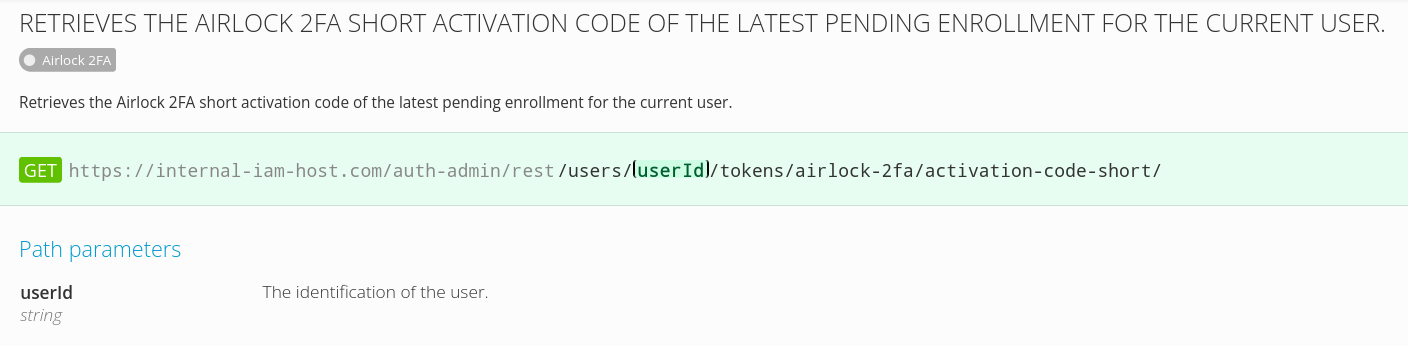
\includegraphics[width=1.0\textwidth]{ressourcen/requestdoc}
		\caption[REST-Dokumentation Request]{Miredot REST-Dokumentation Request}\label{fig:requestdoc}
	\end{center}
\end{figure}
\noindent Zu oberst ist immer der Titel des Requests. Darunter folgt eine Kurze Zusammenfassung. Danach ist der Pfad dargestellt mit der entsprechenden HTTP-Methode.
Zum Schluss folgen die Pfadparamter, was in diesem Fall die User ID ist.
Anschliessend folgt die Response:

\begin{figure}[H]
	\begin{center}
		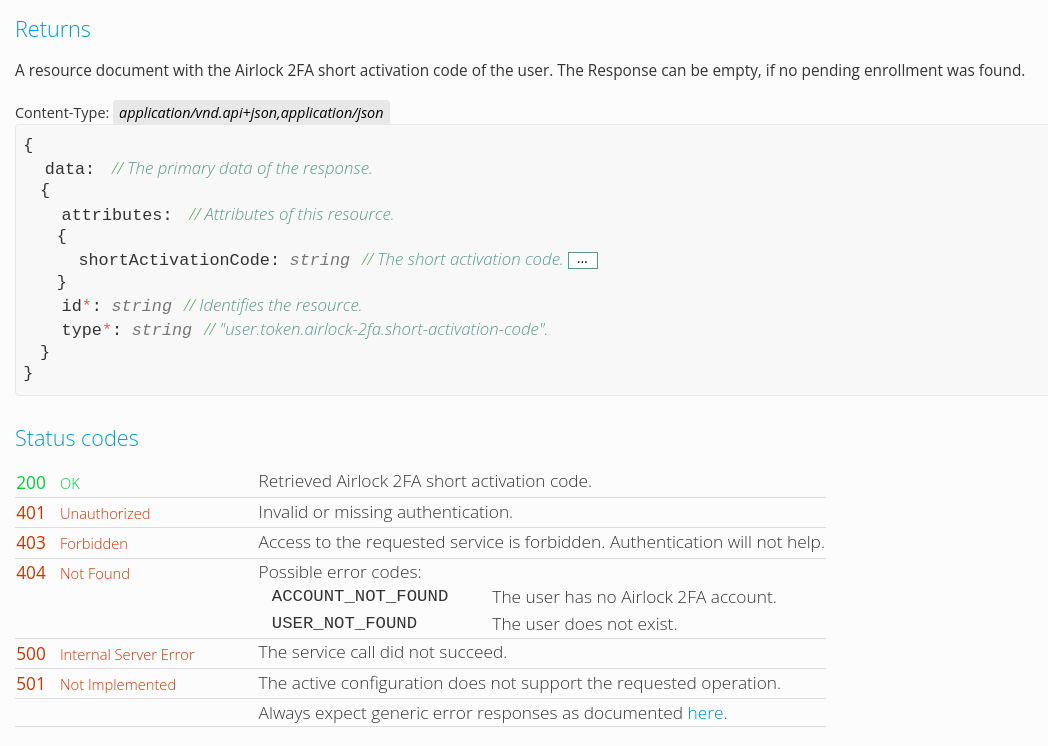
\includegraphics[width=1.0\textwidth]{ressourcen/responsedoc}
		\caption[REST-Dokumentation Response]{Miredot REST-Dokumentation Response}\label{fig:responsedoc}
	\end{center}
\end{figure}

\subsection{Request zu Futurae}




















	\chapter{Kontrollieren}\label{ch:kontrollieren}
Dieses Kapitel bietet Rahmen für die Arbeiten, welche in der IPERKA-Phase <<Kontrollieren>> angefallen sind. In dieser Phase wird die Qualität der Umsetzung geprüft. Es werden alle im Test und Qualitätssicherungskonzept definierten Checks durchgeführt. Falls Fehler auftreten, werden diese behoben.
\section{Durchführen der Tests}
In diesem Abschnitt sind die Ergebnisse der Tests dokumentiert. Die durchgeführten Tests sind im Testkonzept in Kapitel \ref{sec:testkonzept} aufgeführt.
\begin{longtable}{|p{.50\textwidth}|p{.50\textwidth}|}
	\hline
	\textbf{Testdatum} & 18.11.2024 \& 20.11.2024\\
	\hline
	\textbf{Testperson} & Niculin Steiner\\
	\hline
\end{longtable}

\subsection{Unit-Tests}
Alle geschriebenen Unit-Tests sollen erfolgreich durchlaufen.
Folgende 2 Services hatten Logik welche mit Unit-Tests abgedeckt werden musste:
\begin{itemize}
	\item FuturaeAdminApiEnrollmentServiceImpl.java\\
	*Die rot umrahmten Tests wurden im Rahmen der Probe-IPA erstellt.
		\begin{figure}[H]
			\begin{center}
				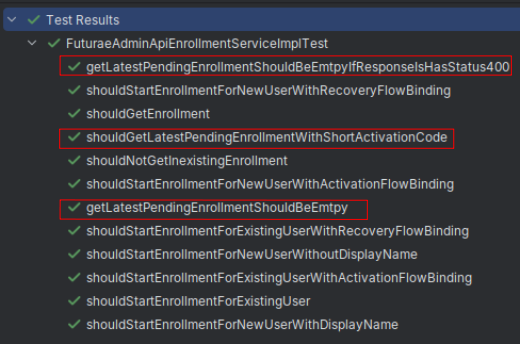
\includegraphics[width=0.8\textwidth]{ressourcen/unittestapi}
				\caption[Unit-Test Resultate FuturaeAdminApiEnrollmentServiceImpl.java]{Unit-Test Resultate FuturaeAdminApiEnrollmentServiceImpl.java}\label{fig:test-admin}
			\end{center}
		\end{figure}
	\item Airlock2FAAdminService.java
		\begin{figure}[H]
			\begin{center}
				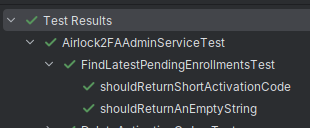
\includegraphics[width=1.0\textwidth]{ressourcen/testadmin}
				\caption[Unit-Test Resultate Airlock2FAAdminService.java]{Unit-Test Resultate Airlock2FAAdminService.java}\label{fig:unittest-api}
			\end{center}
		\end{figure}
\end{itemize}	
\subsection{REST-Integration-Tests}
Alle geschriebenen REST-Integration-Tests sollen erfolgreich durchlaufen.
\begin{figure}[H]
	\begin{center}
		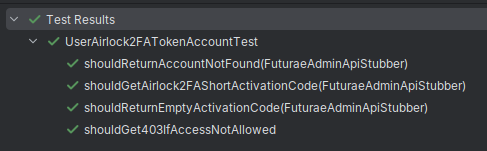
\includegraphics[width=1.0\textwidth]{ressourcen/resttest}
		\caption[REST-Integration-Tests Resultate]{REST-Integration-Tests Resultate}\label{fig:rest-tests}
	\end{center}
\end{figure}
\subsection{UI-Integration-Tests}
Alle geschriebenen UI-Integration-Tests sollen erfolgreich durchlaufen.
\begin{figure}[H]
	\begin{center}
		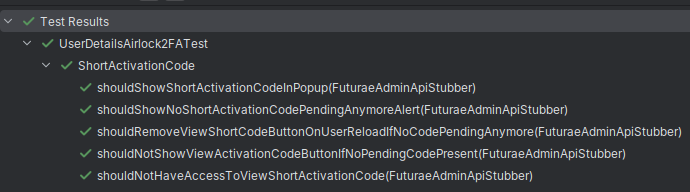
\includegraphics[width=1.1\textwidth]{ressourcen/uitests}
		\caption[UI-Integration-Tests Resultate]{UI-Integration-Tests Resultate}\label{fig:ui-tests}
	\end{center}
\end{figure}
\subsection{Manuelle Tests}
Sowie definiert in Abschnitt \ref{subsec:mtests} werden die manuellen Tests durchgeführt. Der Teststatus wird mit folgenden Symbolen dargestellt:\\

\textcolor{green}{\checkmark}: Test erfolgreich \\

\textcolor{red}{\ding{55}}   : Test fehlgeschlagen\\
\\
In der folgenden Tabelle sind die Resultate der Tests aufgelistet: \newpage
\begin{longtable}{|p{.10\textwidth}|p{.40\textwidth}|p{.40\textwidth}|p{.10\textwidth}|}
	\hline
	\textbf{Testfall} & \textbf{Erwartetes Resultat} & \textbf{Tatsächliches Resultat} &\textbf{Status} \\ \hline
	M1 & Es öffnet sich ein Popup (kein Browserpupop), mit dem Aktivierungscode.  & Es öffnet sich ein Popup (kein Browserpupop), mit dem Aktivierungscode. &  \textcolor{green}{\checkmark} \\ \hline 
	M2 & Der Button wird nicht angezeigt. Der Admin darf auch via einen alternativen REST-Client, wie z.B Postman, den Aktivierungscode nicht bekommen. & Der Button wird nicht angezeigt. Der Admin hat auch via einen alternativen REST-Client, wie z.B Postman, den Aktivierungscode nicht bekommen. & \textcolor{green}{\checkmark} \\ \hline 
	M3 & Der Button wird nicht angezeigt.  &  Der Button wird nicht angezeigt.   & \textcolor{green}{\checkmark} \\ \hline 
\end{longtable}
\noindent Alle Tests konnten erfolgreich durchgeführt werden. Somit funktioniert das neue Feature wie erwartet, und es mussten keine Fehler behoben werden.

\section{Qualitätssicherung}
Die Qualität wurde zum Teil manuell, sowie automatisiert durchgeführt.
\subsection{Manuelle Refactorings}
Um Schreibfehler und andere unschönheiten im Code zu finden und zu verbessern wurde nach dem Implementieren, der ganze, neu geschriebene Code nochmals durchgegangen und kleine Findings wurden direkt behoben oder refactored.

\subsection{Automatisierte Code-Analyse}
Die Qualitätssicherung wurde auch während der Entwicklung fortlaufend sichergestellt. Jeder Commit, welcher auf Gerrit landet löst automatisch die Build Pipeline auf dem Jenkins aus. Diese führt neben den ganzen Code-Tests auch statische Code-Analysen durch. Diese sind:
\begin{itemize}
	\item SpotBugs
	\item PMD
	\item CheckStyle
\end{itemize}
\newpage
Resultate des letzten, finalen Commits:
\begin{figure}[H]
	\begin{center}
		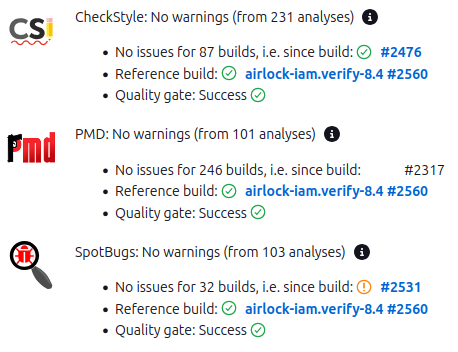
\includegraphics[width=0.8 \textwidth]{ressourcen/codeana}
		\caption[Resultate Code-Analyse]{Resultate der Code-Analyse Tasks auf Jenkins}\label{fig:codeana}
	\end{center}
\end{figure}
\noindent Wie im obigen Bild zusehen, sind alle Checks für diesen Build erfolgreich durchgelaufen. Dies bedeutet die Qualitätssicherung ist so gut wie möglich sichergestellt.

	\chapter{Auswerten}\label{ch:auswerten}
    \printglossaries
    \renewcommand*{\listfigurename}{Abbildungsverzeichnis}
\listoffigures
% Structure:
% \begin{figure}
% \captionsetup{textformat=empty, labelformat=empty} -> to hide the caption beneath the image
% \includegraphics[format]{resource}
% \caption[<caption> (<cite source>) | caption (Eigene Darstellung)]{<caption>}\label{fig:<label>}
% \end{figure}
\

\end{document}
